\section{General}

This chapter details the experimental investigations conducted on complex LSF wall systems under ambient conditions. Despite the advancements in numerical models, experiments are necessary to determine the ambient load carrying capacity and the robustness of developed FE models to predict the axial load carrying capacity of the complex LSF wall systems. Also, the capacity of walls at ambient temperatures are required to conduct full-scale fire tests under load bearing conditions in which as a percentage of the ambient axial capacity of the wall system is applied during fire tests. Therefore, experimental investigations were carried by conducting ambient capacity tests and the ambient load carrying capacity of the complex LSF wall specimens were determined. Tensile coupon tests were also conducted on the steel studs to determine the yield strength of the studs which will later be used for the numerical analyses and parametric studies.  

\section{Ambient Capacity Test Setup}

Ambient capacity tests are used to determine the axial load carrying capacity to be used for the fire test in accordance with AS 1530.4. However, the testing procedures to determine the ambient capacity is not detailed clearly in the aforesaid standards. Therefore the tests were conducted similar to full-scale fire tests without the fire load. The ambient capacity tests were conducted on a specially built test frame which can accommodate specimens up to 3 m \(\times\) 3 m in external dimensions. The test frame consists of two Universal Columns (UC's) fixed to the strong floor. At the top the columns are connected through a Welded Beam (WB) and at the bottom through a Universal Beam (UB) resting on the floor. Individual hydraulic ramps were used to load the test wall at the stud locations and are placed on the bottom Universal Beam (UB). The test specimens are loaded from the bottom rather than the top for the ease of experimental set up. LSF wall specimens are constructed on a mounting table held on to the ground. After construction, the test specimens are loaded into the test frame using forklift and Electric Overhead Travelling (EOT) crane. Linear Variable Displacement Transducers (LVDT's) were used to measure the axial displacement and lateral deflection at various locations during the test. The axial displacements were measures at the bottom loading plate near the rams. Lateral deflection was measured at three locations in critical studs which include the 750 mm from the top and bottom of the specimen and also at mid-height of the specimen. Details of a typical test specimen and the loading frame is shown in \Cref{fig:typical-ambient}.
\begin{figure}[!htbp]
	\centering
		\begin{tabular}{c}
			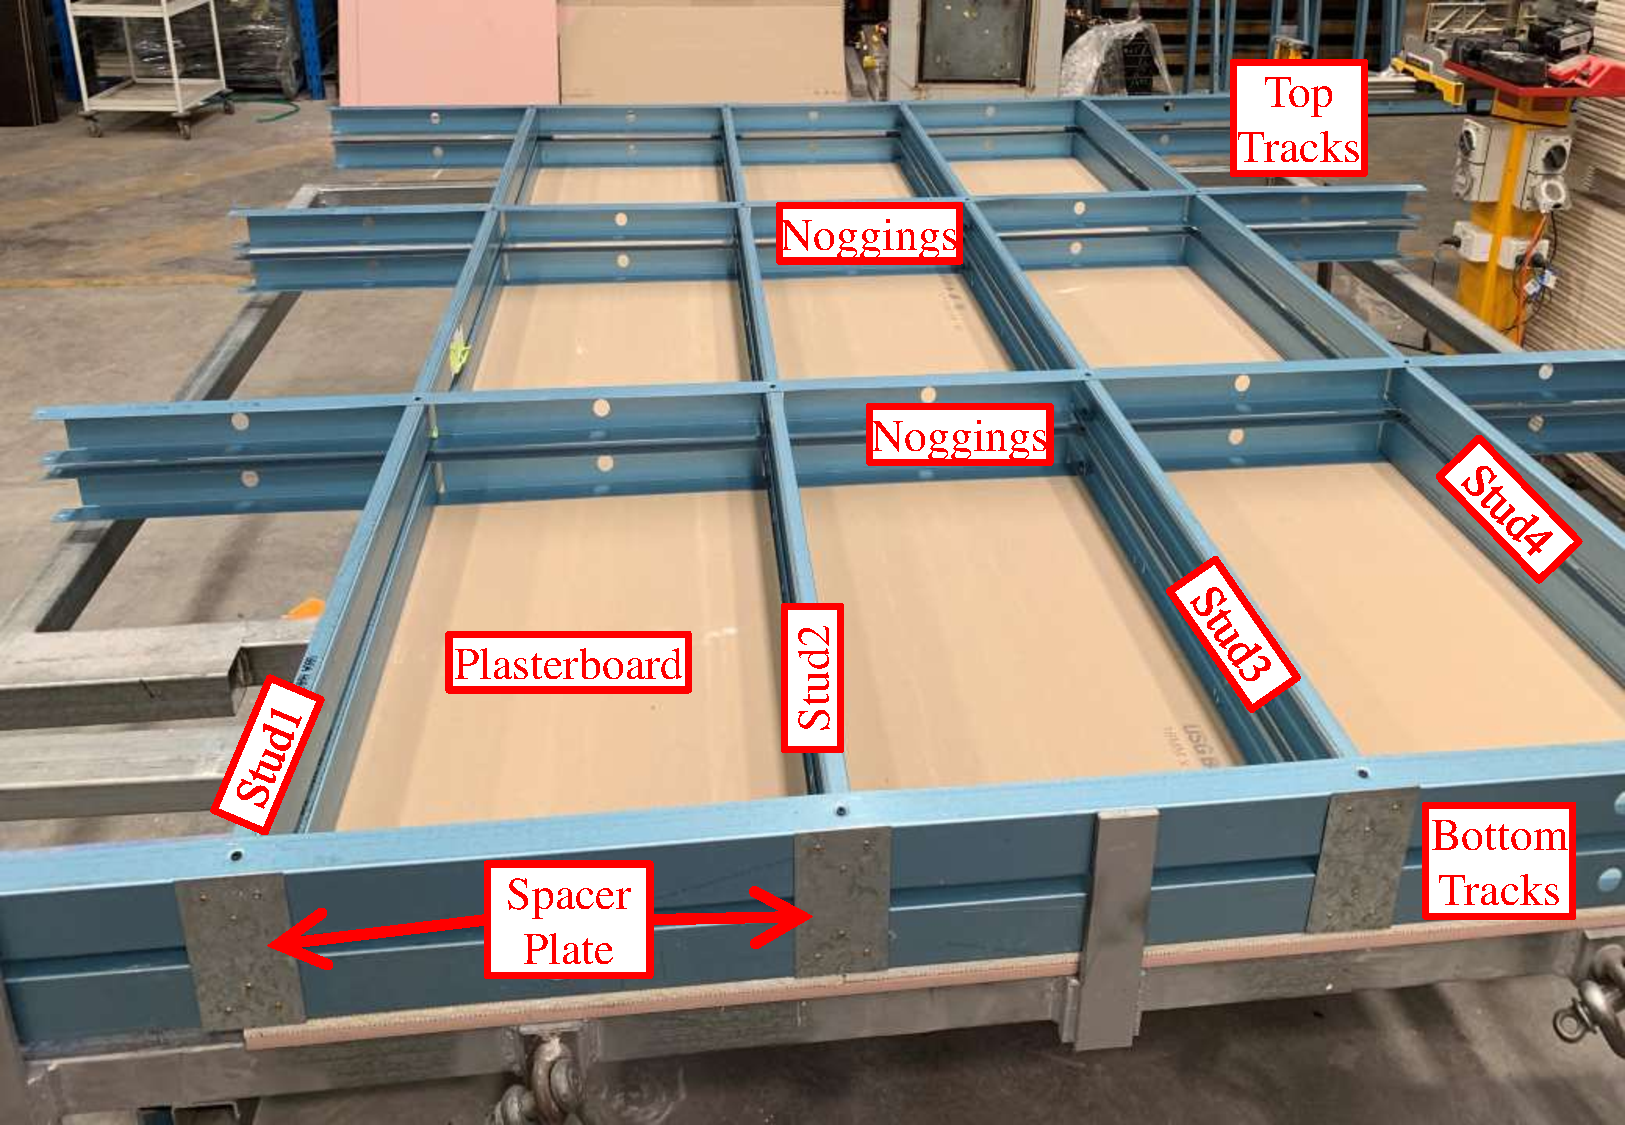
\includegraphics[scale=0.3]{ambient_construction.pdf} \\
			(a) \\
			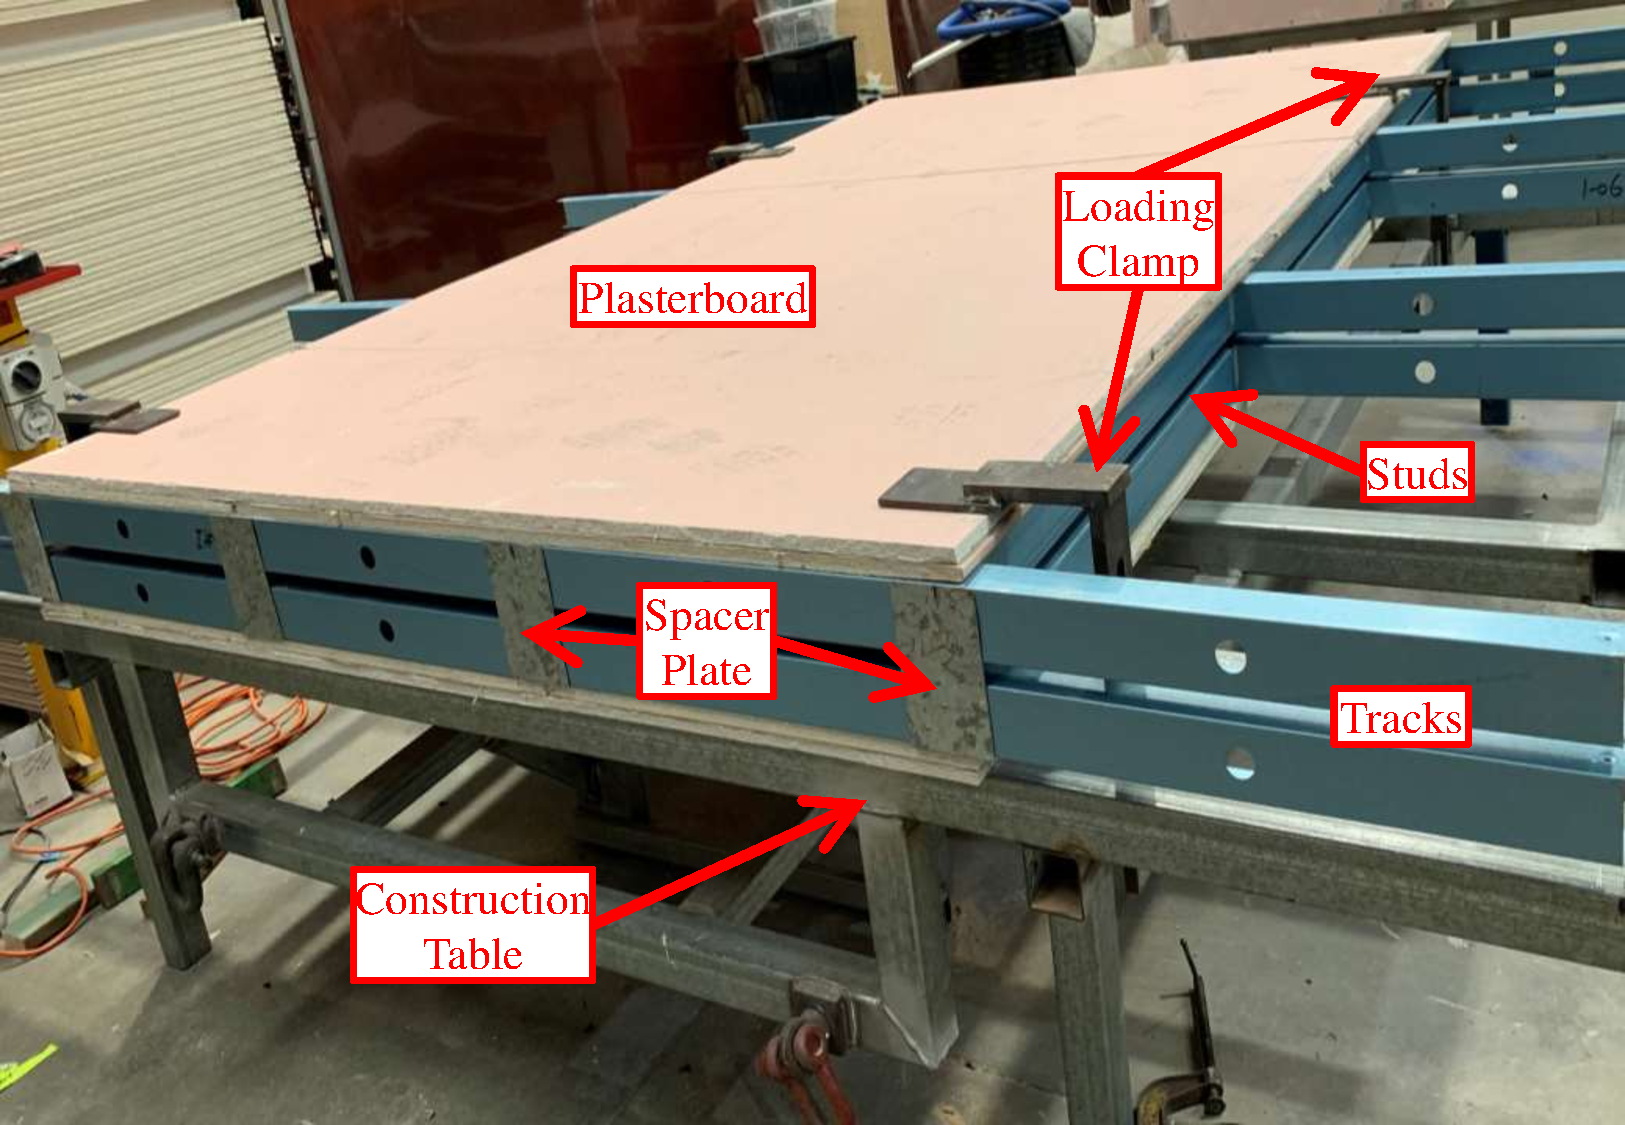
\includegraphics[scale=0.3]{ambient_finished.pdf} \\ 
			(b)  \\
			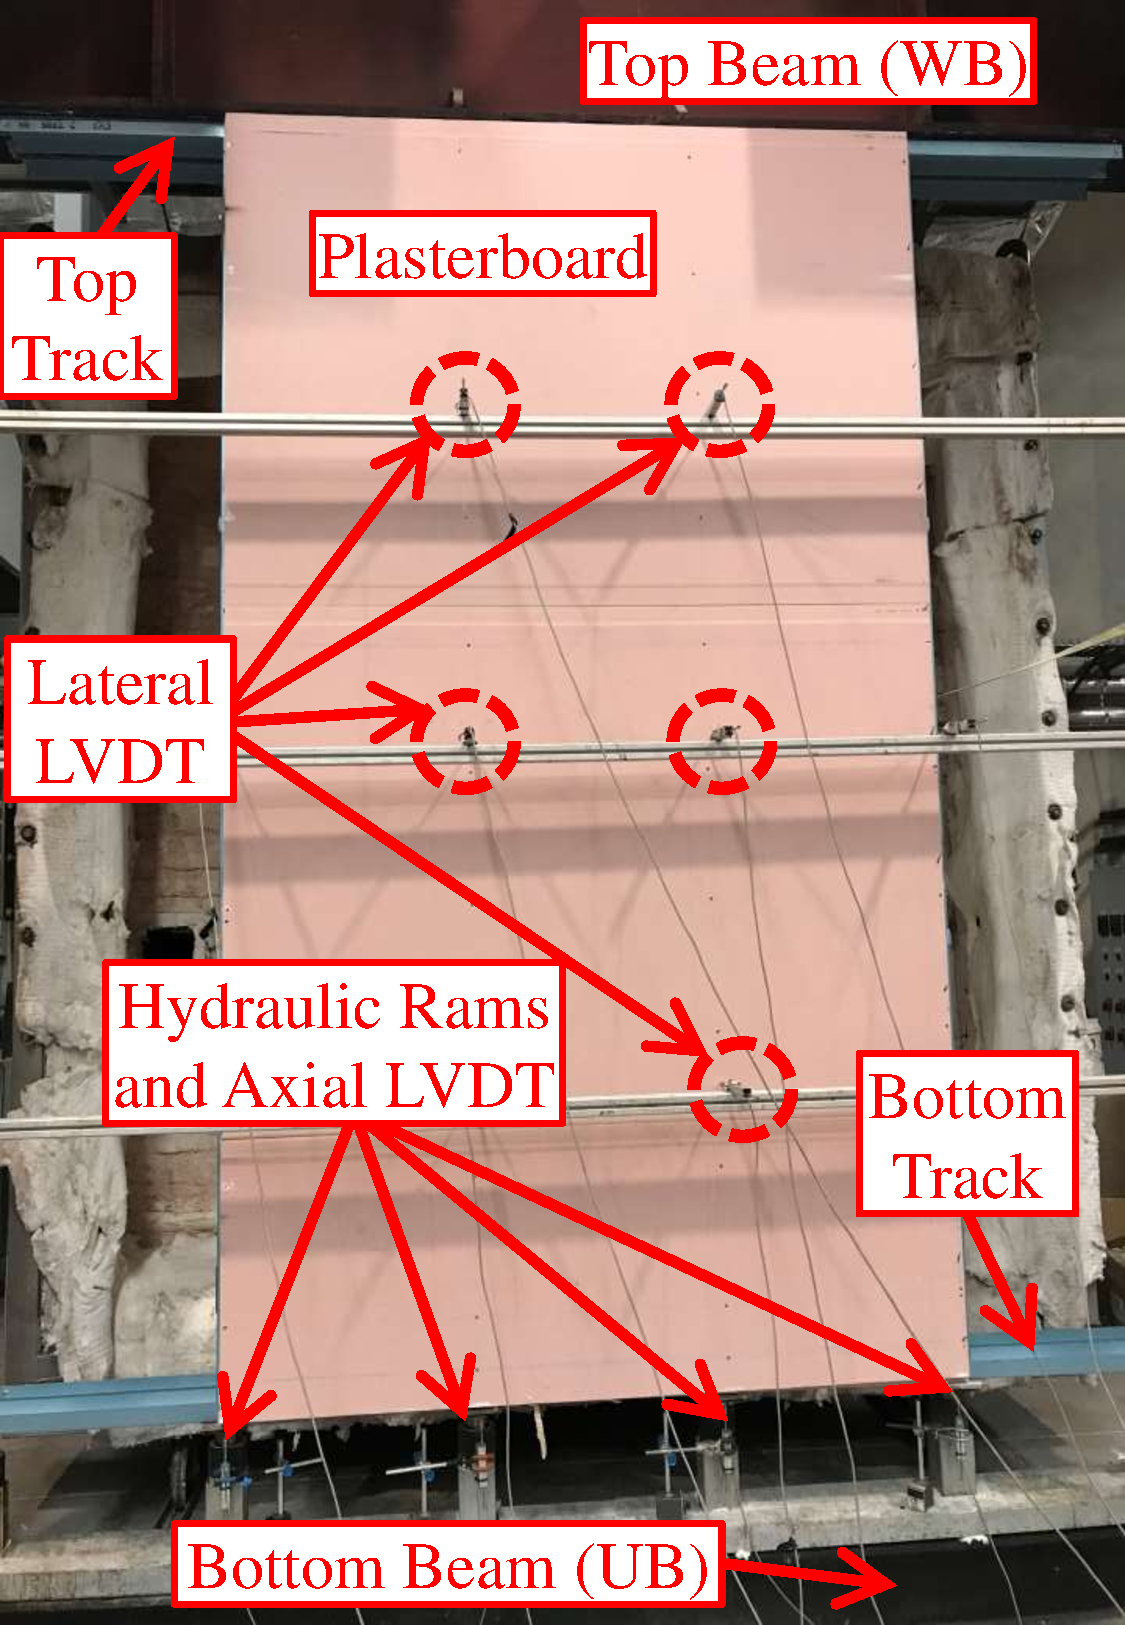
\includegraphics[scale=0.25]{typical_ambient.pdf}\\
			(c)  \\ 
		\end{tabular} 
		\caption{Typical experimental set-up of ambient stud wall (a) Construction of the test wall (b) Finished test wall (c) Loaded test wall}
		\label{fig:typical-ambient}
\end{figure}

A summary of the ambient capacity test conducted as a part of this research study is presented in \Cref{tab:ambient-test-specimens}. All the test specimens had Lipped Channel Sections (LCS) as studs made of G550 steel manufactured by Bluescope with a minimum guaranteed yield strength of 610 Mpa. The steel studs had pre punched holes drilled on them at required positions for easier construction. Buildex M6.0 \(\times\) 15 GX Ca smooth top GA point steel frame screws were used to connect the steel studs to the tracks and noggings. Unlipped Channel Sections (UCS) were used for the top and bottom tracks and pre punched holes were made in the flanges of the tracks and corresponding locations to fix the studs. UCS were used as noggings at 1 m intervals in all the tests but for Test-AT5. However, the UCS noggings were replaced by omega noggings and details about the same are provided in the corresponding section.
\begin{table}[!htbp]
	\centering
	\caption{Ambient test panel details}
	\begin{tabular}{cccccc}
		\toprule
		\multicolumn{1}{m{2.4em}}{\centering{Test Name}} & 
		\multicolumn{1}{m{5.6em}}{\centering{Description}} & 
		\multicolumn{1}{m{2.85em}}{\centering{Stud Depth (mm)}} & 
		\multicolumn{1}{m{2.85em}}{\centering{Cavity Depth (mm)}} & 
		\multicolumn{1}{m{5em}}{\centering{Stud Thickness (mm)}} & 
		\multicolumn{1}{m{3em}}{\centering{No of Studs}} \\
		\midrule
		AT1  & Double Stud & 90 & 200 & 0.95 & 4 \\
		AT2  & Double Stud & 90 & 200 & 0.75 & 4 \\
		AT3  & Double Stud & 90 & 200 & 0.75 & 6 \\
		AT4  & Double Stud & 70 & 160 & 0.95 & 4 \\
		AT5  & Staggered Stud & 90 & 200 & 0.95 & 6 \\
		\bottomrule
	\end{tabular}%
	\label{tab:ambient-test-specimens}%
\end{table}%

All the test specimens were lined with two layers of 16 mm fire rated gypsum plasterboard. The plasterboards were connected to the stud flanges through D type 10 GA self-piercing screws. The first layer of plasterboard was fixed to the studs using 32 mm long screws while the second layer was fixed using 45 mm long screws. The plasterboards joints were not seals with joint compound as the corresponding effect on ambient load carrying capacity is negligible. The plasterboards were fixed with a screw spacing of 200 mm at joints in a staggered manner while linear arrangement with 300 mm spacing was adopted at the edges and at plasterboard centres. A 60 mm gap for first layer and 80 mm gap for second layer of plasterboard was provided to prevent plasterboards being screwed on to the top and bottom tracks to allow for axial compression expansion during the tests. Description about the variations in the individual ambient capacity tests and their corresponding results are discussed next.

\section{Ambient Test-AT1}\label{sec:AT1}

The first ambient capacity test was conducted on double stud LSF wall with 90 mm studs. Grade 550 steel with dimensions of 90\(\times\)36\(\times\)7\(\times\)0.95 were used as studs. 90 mm unlipped channel sections were used as noggings at 1 m intervals. The noggings were connected to the studs through slots made on the webs of the UCS. Top and bottom of the test specimen were connected through 90 mm unlipped channel sections. It is to note that, the test wall had two rows of studs separated by a 20 mm gap between the studs as shown in \Cref{fig:AT1-plan}. Four studs were used for the ambient capacity test and the edge studs were strengthened to induce failure on the middle studs as the plasterboard provide effective in-plane restraints only to the middle studs. The height of the specimen was 3 m while the width was 1.8 m.  
\begin{figure}[!htbp]
	\centering
			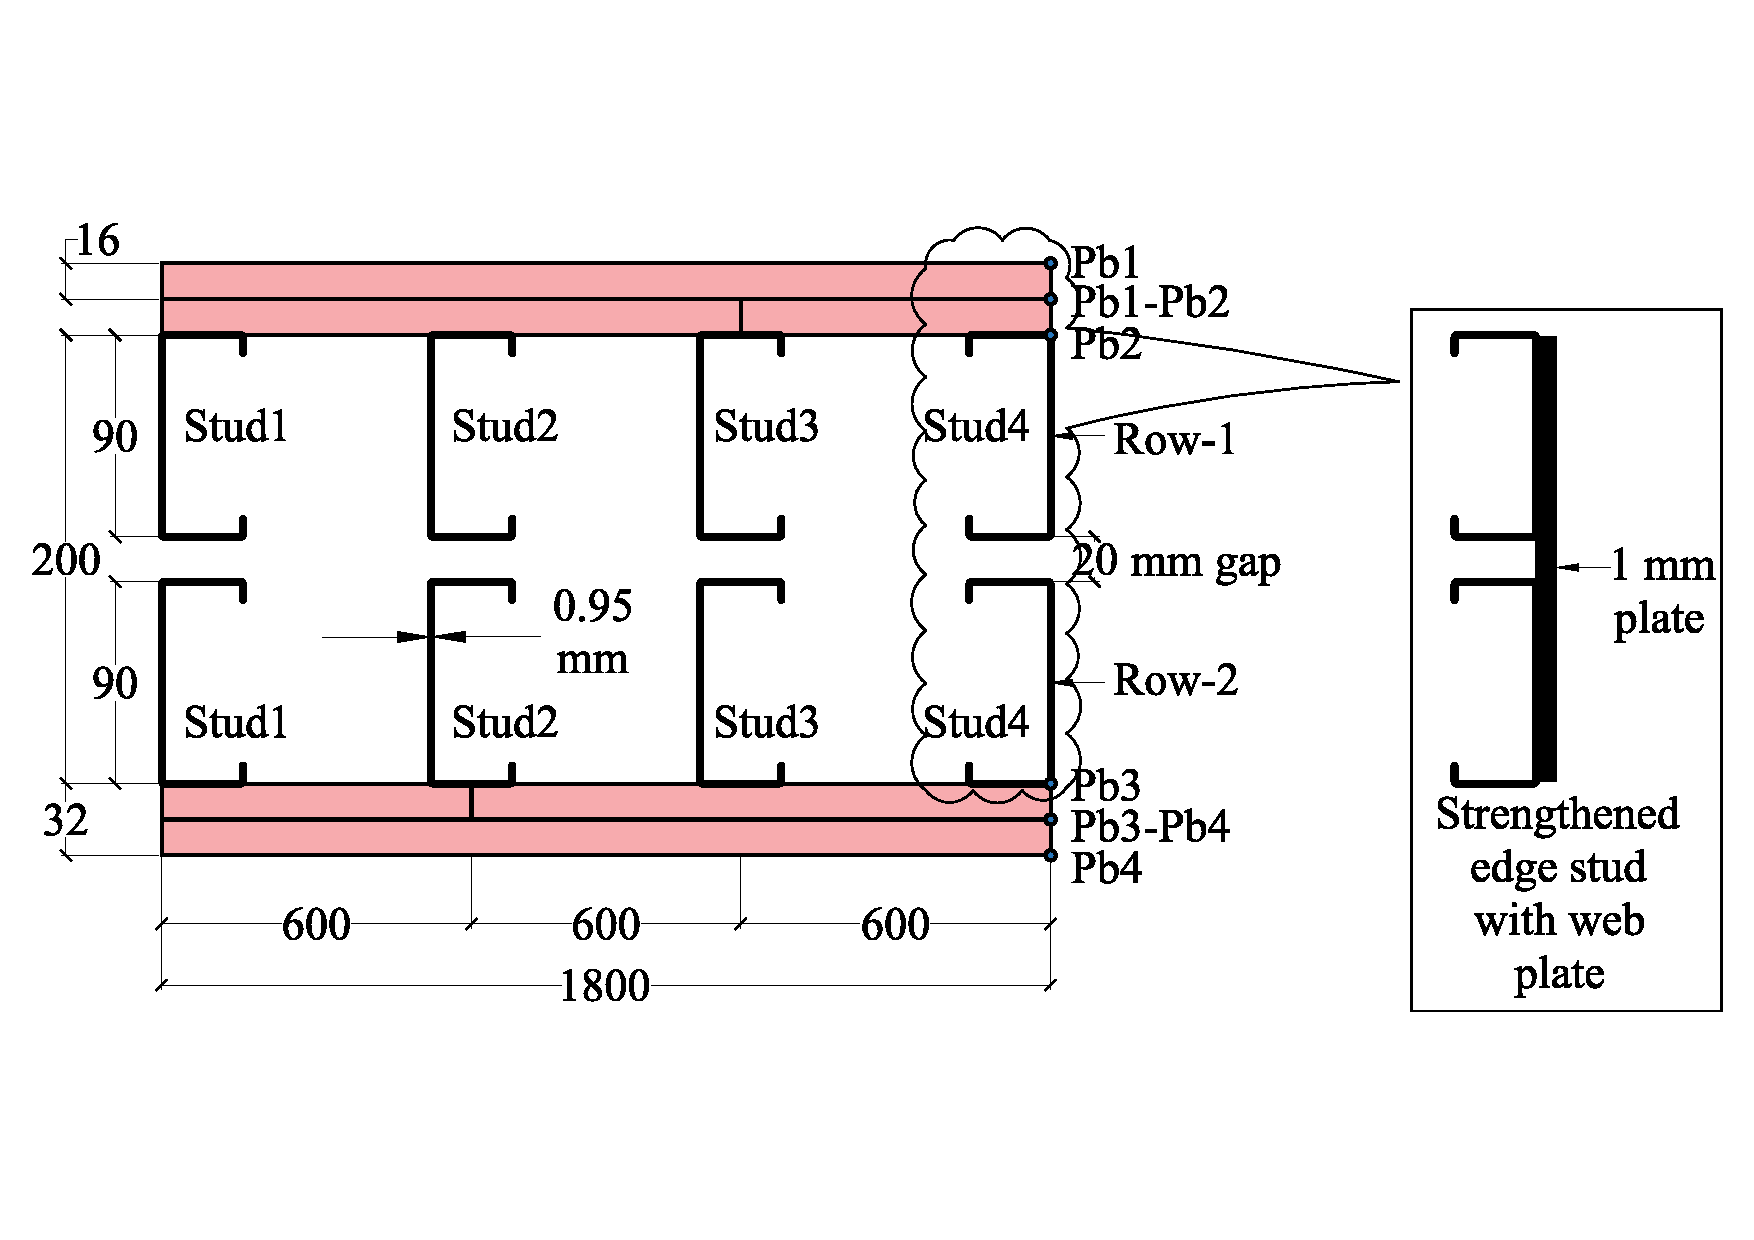
\includegraphics[scale=0.25]{AT1-plan.pdf}\\
		\caption{Test-AT1 configuration}
		\label{fig:AT1-plan}
\end{figure} 

Firstly, the test specimen was loaded to 10\% of the predicted ambient load carrying capacity for two cycles before commencing the ambient capacity test to relieve internal stresses developed in the specimen due to the construction process. After this the ambient capacity test was carried out by applying the load on the geometric centre of the studs through individual rams as shown in \Cref{fig:typical-ambient}.
\begin{figure}[!htbp]
	\centering
			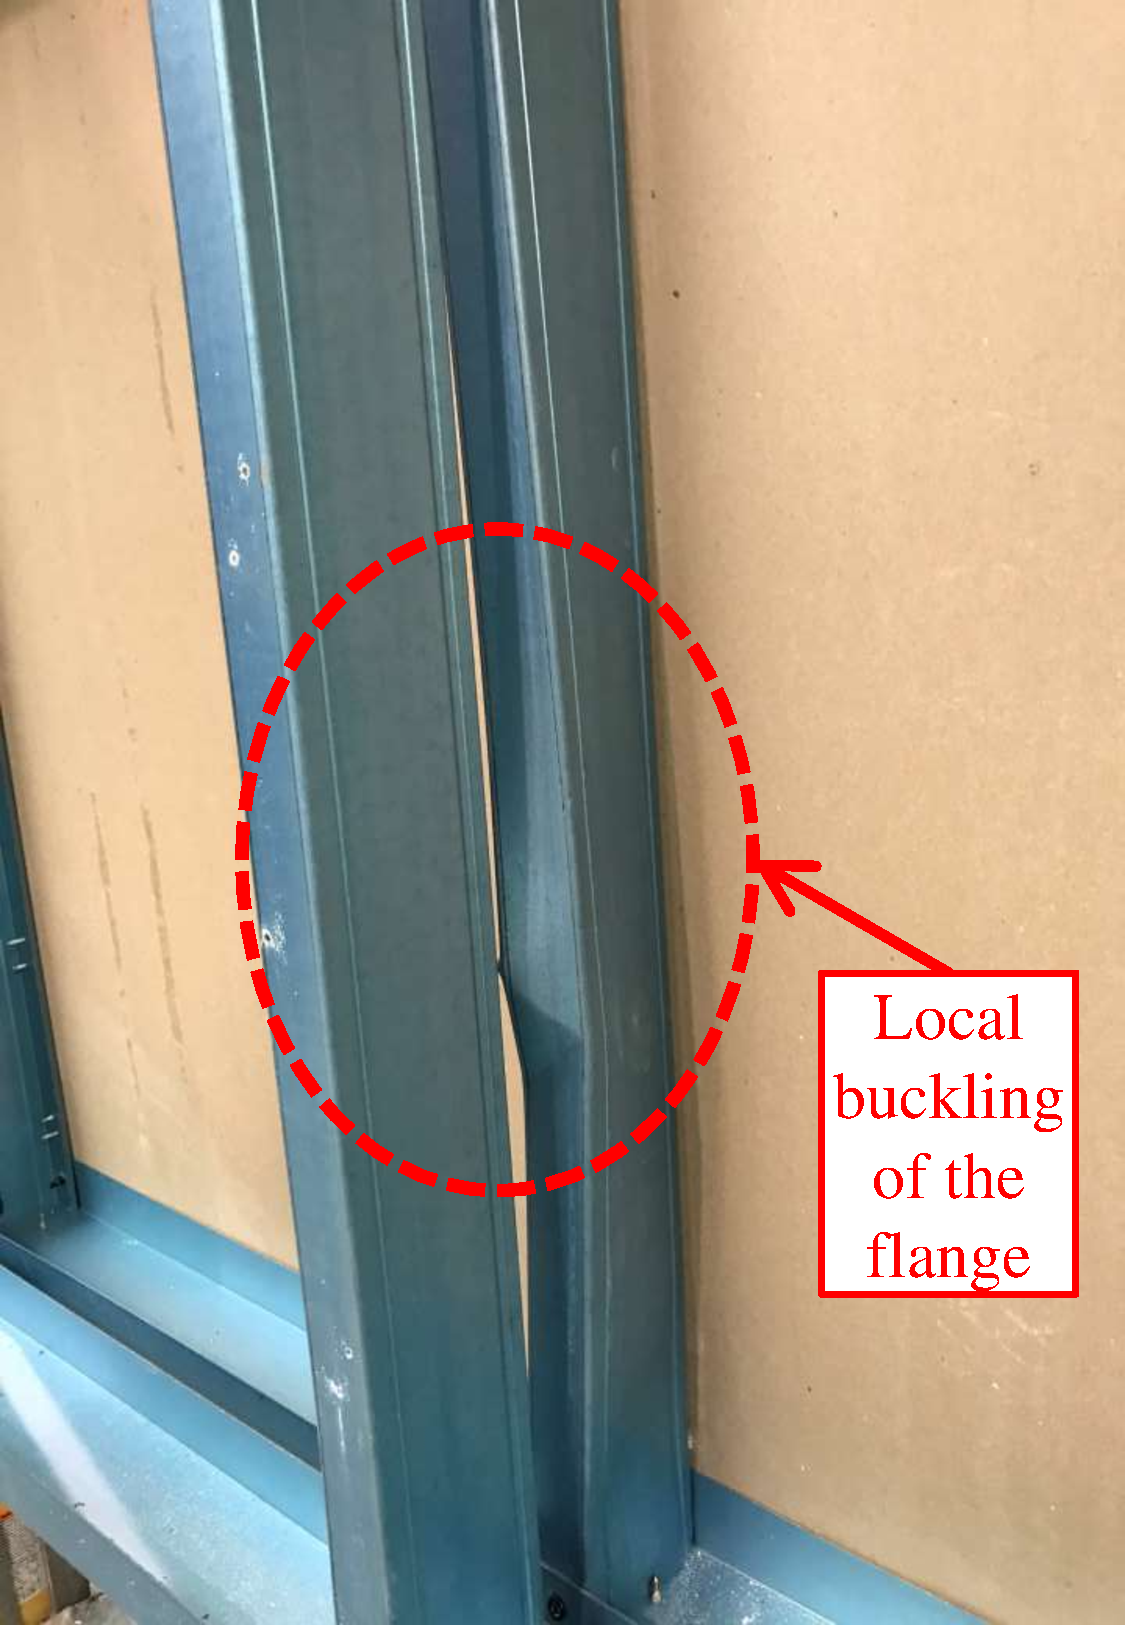
\includegraphics[scale=0.2]{AT1-buckling.pdf}\\
		\caption{Local compressive failure in test-AT1}
		\label{fig:AT1-buckling}
\end{figure} 

The ambient Test-AT1 resulted an ultimate capacity of 73 kN. Local buckling of the studs was observed in the flanges as shown in \Cref{fig:AT1-buckling}. No pull-out of the plasterboard screws were observed during the ambient capacity test. The load versus axial displacement and load versus lateral deflection curves are shown in Figures~\ref{fig:AT1-results}~(a)~and~(b). The maximum axial displacement was recorded as 13.28 mm in Stud2. Generally, in ambient capacity tests the application of load is  continued till the ultimate failure load is reached after which the applied load transferred to the studs in which buckling has not been initiated. This results in excessive post-buckling failures in some studs during the ambient capacity tests. Post-buckling failures are noticeable in Stud4 due to the additional load acting upon them as Stud2 has already buckled initially. This is evident in the load versus axial displacement curve where a maximum of 25.78 mm displacement was observed in Stud4 as shown in \Cref{fig:AT1-results}~(a).
\begin{figure}[!htbp]
	\centering
		\begin{tabular}{cc}
			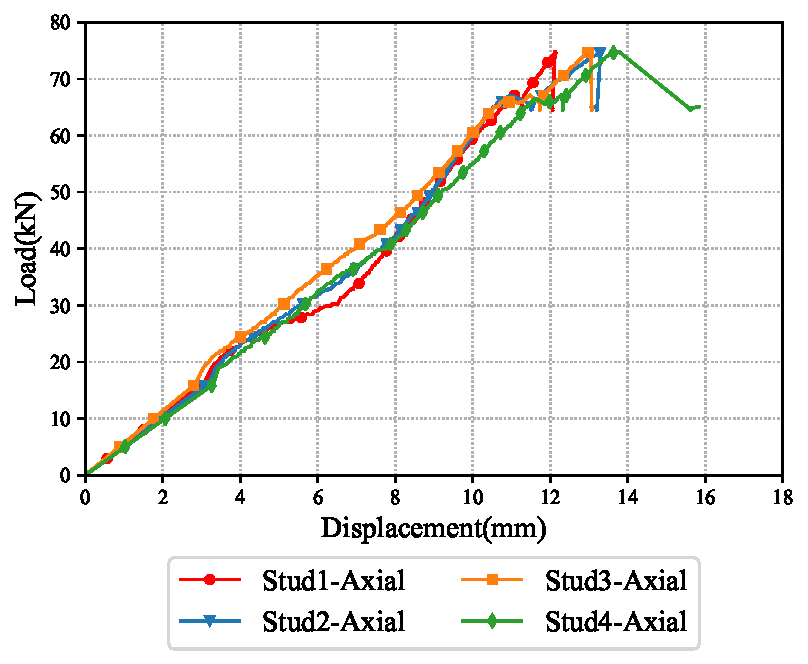
\includegraphics[width=6.5cm,height=6cm]{AT1-Load-Axial-Corrected.pdf} & 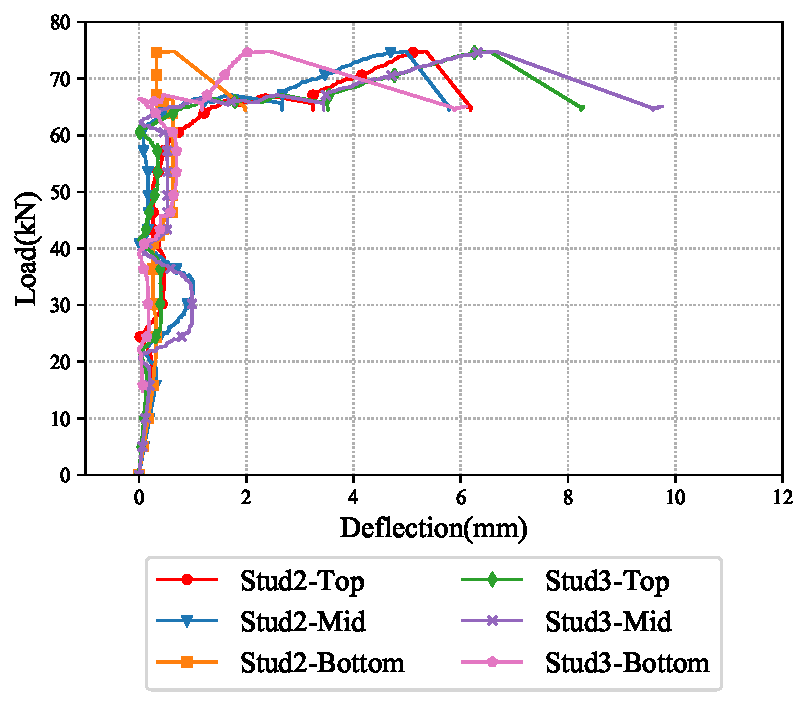
\includegraphics[width=6.5cm,height=6cm]{AT1-Load-Lateral-Corrected.pdf} \\ 
			(a) & (b)  \\ 
		\end{tabular} 
		\caption{Test-AT1 results - (a) Axial displacement and (b) Lateral deflection versus applied axial load}
		\label{fig:AT1-results}
\end{figure}

\section{Ambient Test-AT2}

The second ambient capacity test was conducted on thinner stud sections (0.75 mm) with stud dimensions of 90\(\times\)36\(\times\)7\(\times\)0.75 mm. This test was conducted to determine the effect of thickness in the axial compression capacity of double stud walls. The test specimen was constructed and tested with four studs. The stud depth, flange width and the lip depth were same in comparison with test AT1 while the thickness of the studs were reduced from 0.95 mm to 0.75 mm. Testing procedure was similar to the one adopted in AT1. After loading the specimen to the test frame the test wall was loaded till the ultimate failure in studs. Test-AT2 resulted in a maximum axial compression capacity of 47.08 kN. Local compressive failure in the flanges of Stud2 was noticed as shown in \Cref{fig:AT2-buckling}. No crack in plasterboards or pull out failure of screws at plasterboard connections were noticeable on both sides after the test.  
\begin{figure}[!htbp]
	\centering
			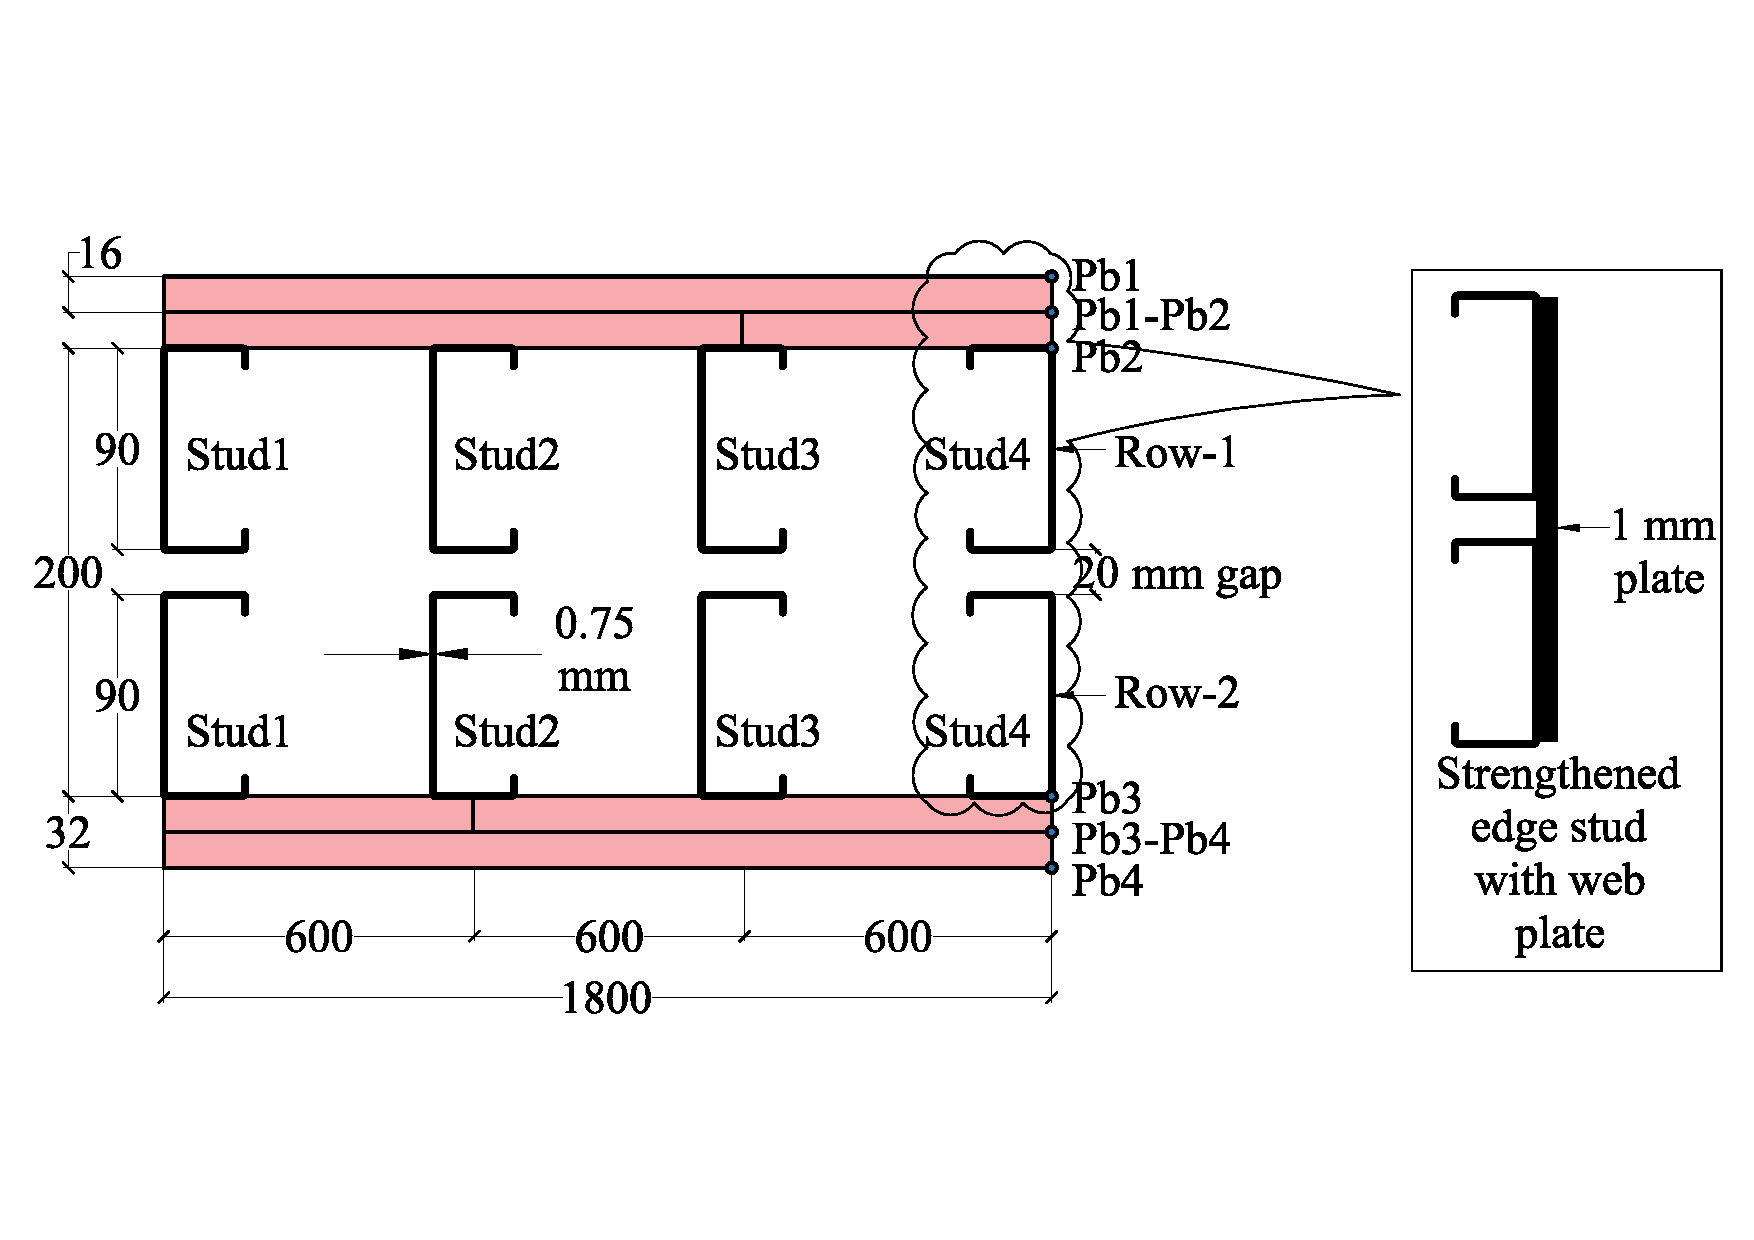
\includegraphics[scale=0.25]{AT2-plan.pdf}\\
		\caption{Test-AT2 configuration}
		\label{fig:AT2-plan}
\end{figure}  
\begin{figure}[!htbp]
	\centering
			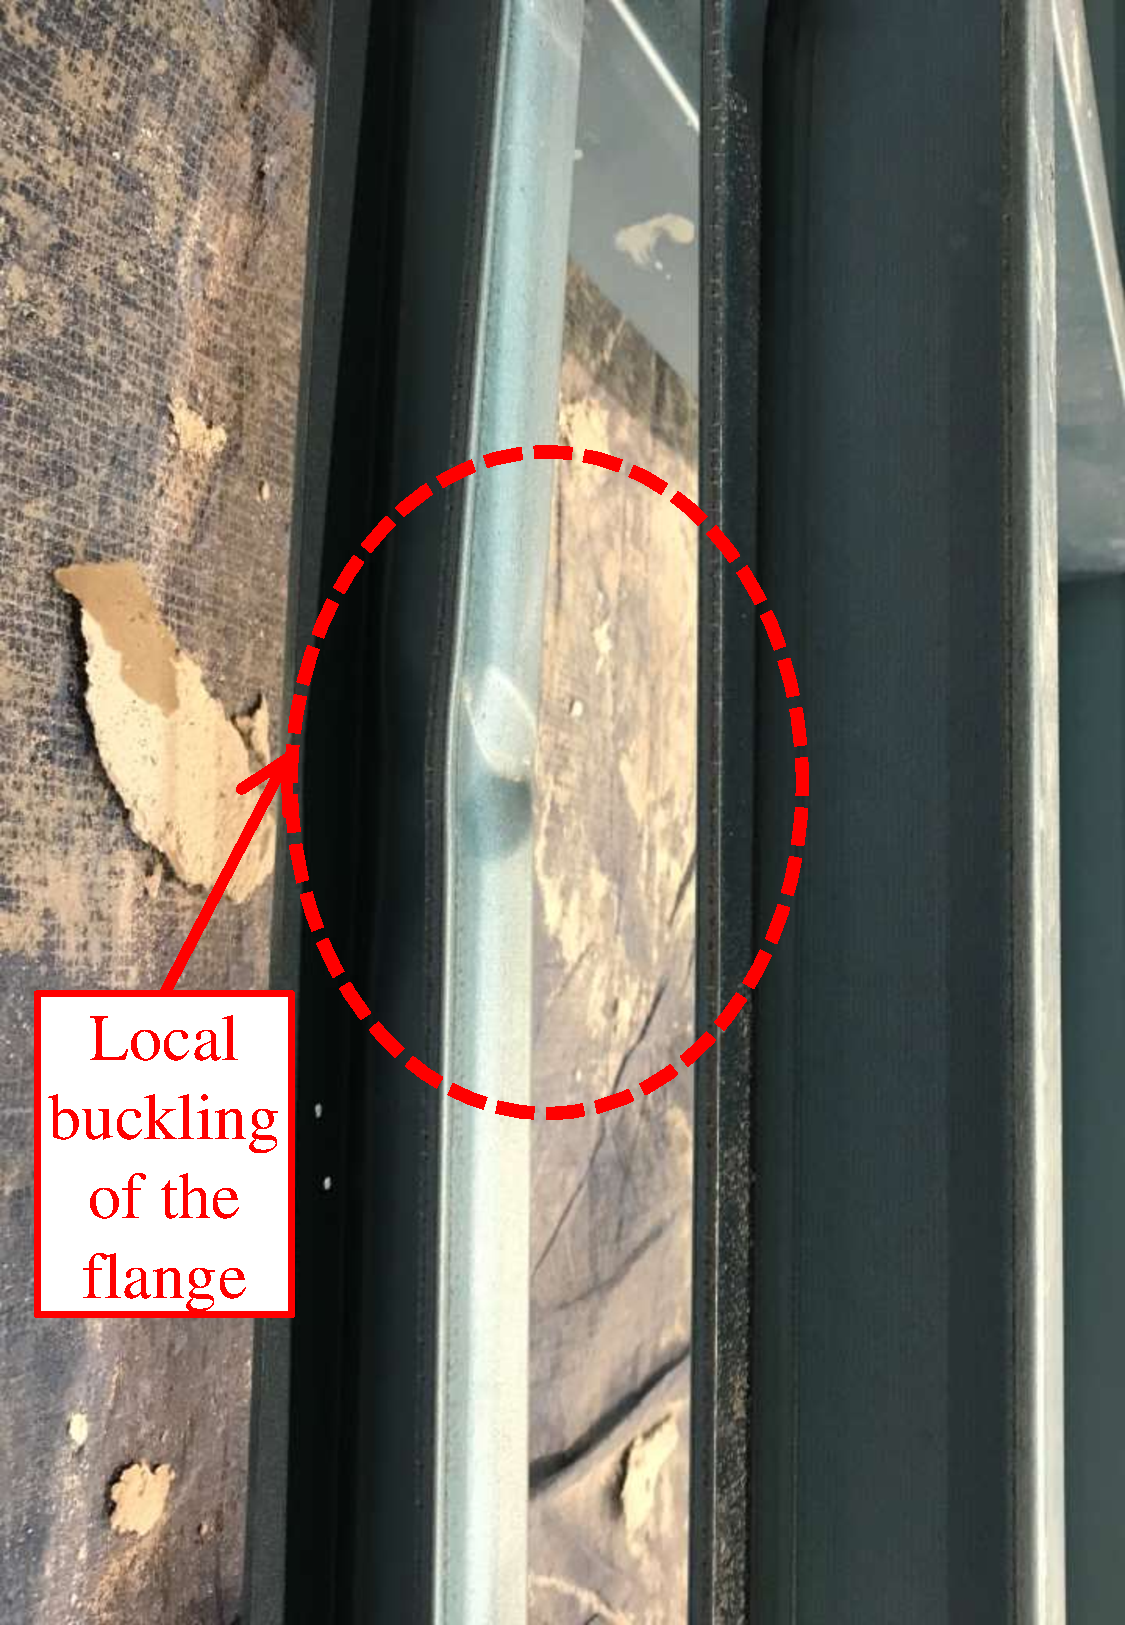
\includegraphics[scale=0.25]{AT2-buckling.pdf}\\
		\caption{Local compressive failure in test-AT2}
		\label{fig:AT2-buckling}
\end{figure}
\begin{figure}
	\centering
		\begin{tabular}{cc}
			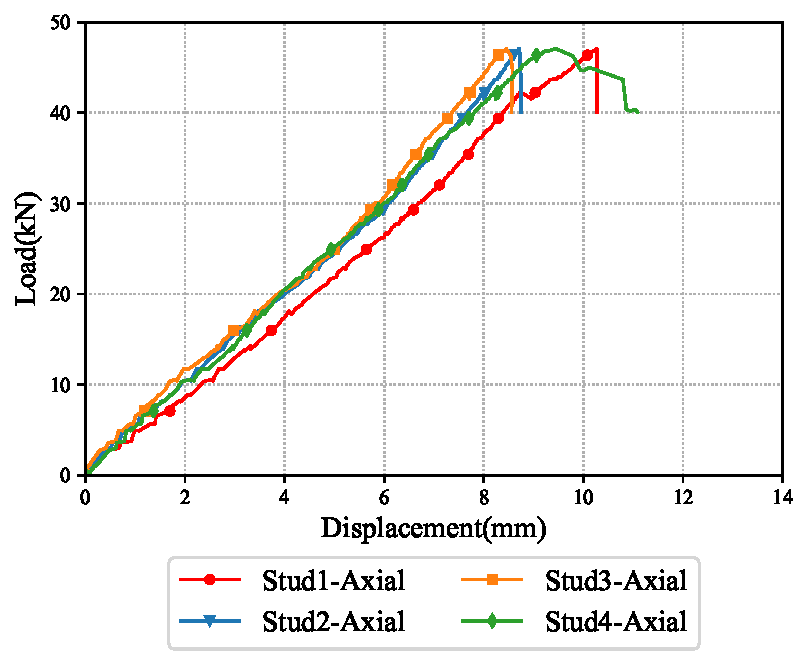
\includegraphics[width=6.5cm,height=6cm]{AT2-Load-Axial-Corrected.pdf} & 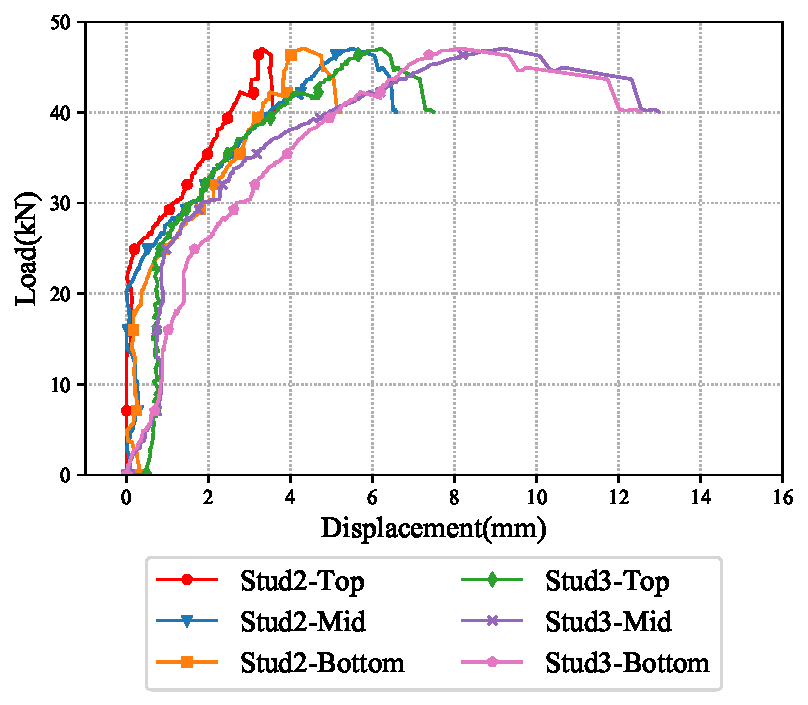
\includegraphics[width=6.5cm,height=6cm]{AT2-Load-Lateral-Corrected.pdf} \\ 
			(a) & (b)  \\ 
		\end{tabular} 
		\caption{Test-AT2 results - (a) Axial displacement and (b) Lateral deflection versus applied axial load}
		\label{fig:AT2-results}
\end{figure}
Figures~\ref{fig:AT2-results}~(a)~and~(b) shows the axial displacement and lateral deflection curves from the ambient capacity Test-AT2. The maximum axial displacement recorded was 10.27 mm in all tests as shown in \Cref{fig:AT2-results}~(a). However, as explained in the previous Test-AT1, the corner stud experience post buckling load resulting in an axial displacement of 16.51 mm. A lateral deflection of 25.18 mm at Stud3-Bottom was recorded as shown in \Cref{fig:AT2-results}~(b). The deflections are more in comparison with Test-AT1. This is because of thin stud section used in this test which has a higher slenderness ratio in comparison with Test-AT1.

\section{Ambient Test-AT3}

The third ambient capacity test was similar to Test-AT2 but with six studs. This test was conducted with six studs to verify the axial compression capacity of double studs LSF wall Test-AT2. \Cref{fig:AT3-plan} shows the test configuration of double stud LSF wall tested with six studs. It is to note that, despite having six studs in the test wall the effective in-plane restraints provided by the plasterboards is applicable only to four studs in the middle leaving the end two studs with partial restraint. This is because the effective distance between the middle two studs are 300 mm on either sides while the effective distance in only 300 mm on one side for the end studs. Similar to the previous ambient capacity tests, after the initial pre-loading cycle, the ambient capacity of the test wall was determined by applying axial compressive load to the individual studs. The test wall resulted in a maximum axial compression capacity of 39.42 kN. Local bearing failure was observed in the end stud as shown in \Cref{fig:AT3-buckling}.
\begin{figure}[!htbp]
	\centering
			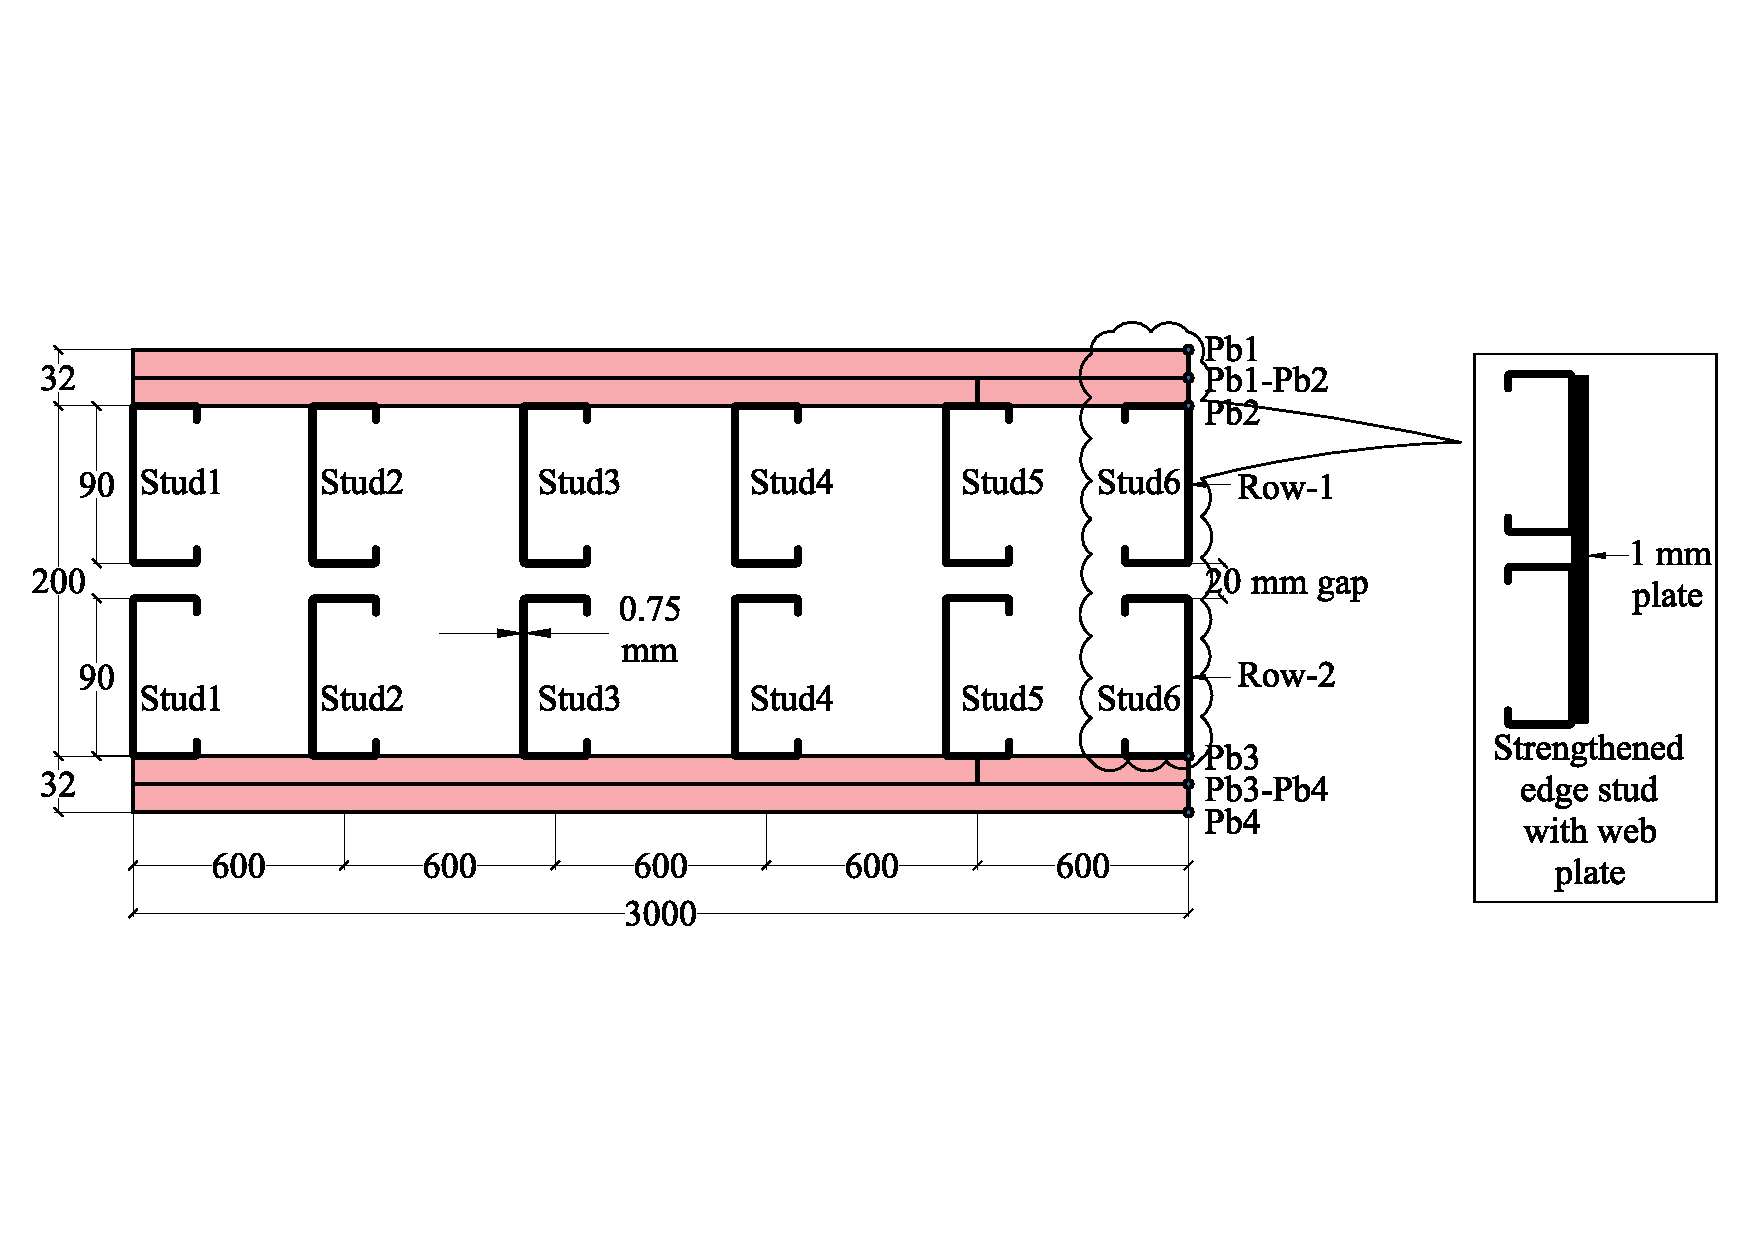
\includegraphics[scale=0.25]{AT3-plan.pdf}\\
		\caption{Test-AT3 configuration}
		\label{fig:AT3-plan}
\end{figure}  
\begin{figure}[!htbp]
	\centering
			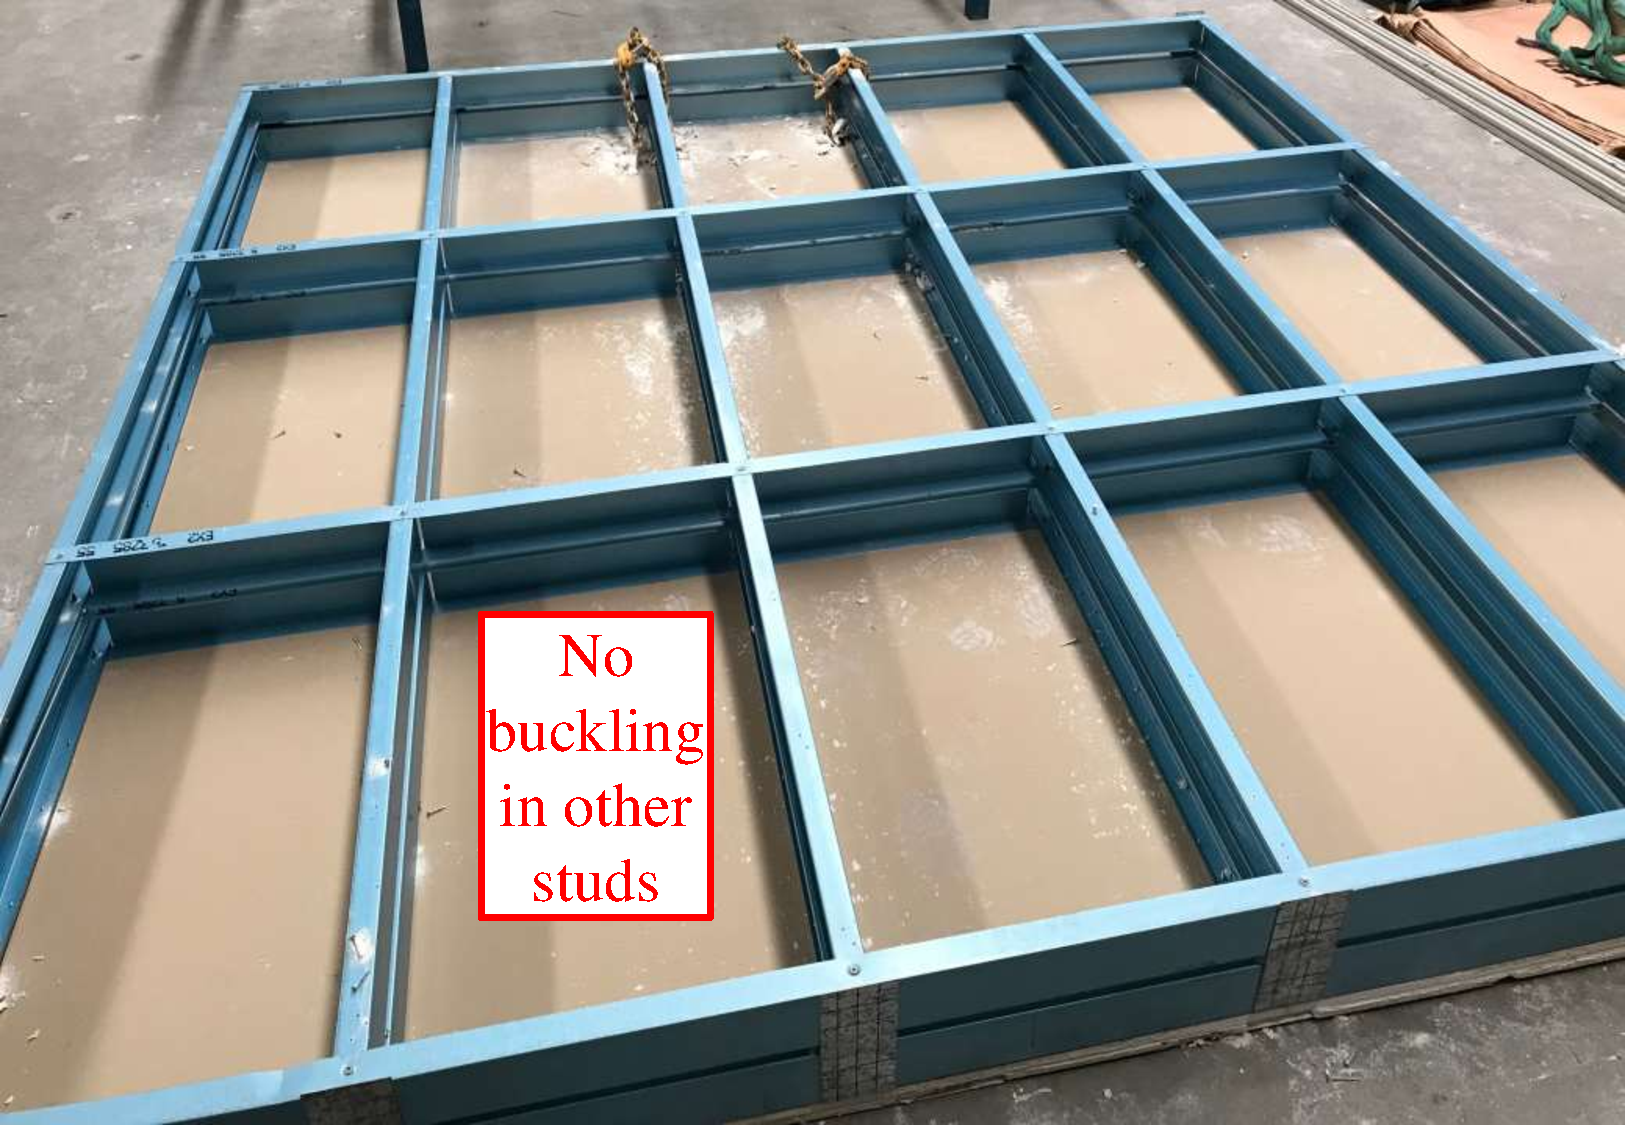
\includegraphics[scale=0.3]{AT3-buckling.pdf}\\
		\caption{Local bearing failure in test-AT3}
		\label{fig:AT3-buckling}
\end{figure}

The axial displacement and lateral deflection curves are presented in \Cref{fig:AT3-results} (a)~and~(b). Maximum axial displacement of 9 mm was recorded in Stud2 and a maximum lateral deflection of 6.41 mm was observed at Stud4-Bottom. In comparison with Test-AT2 the axial compression capacity was 7.66 kN lesser. This was due to the bearing failure experienced in the end studs in comparison to local buckling failure in Test-AT2. The plasterboards do not provide effective lateral restraints to the end studs in comparison to the middle studs causing this failure. However, the axial displacement and lateral deflections were similar both Tests-AT2 and AT3 but for the end studs as shown in \Cref{fig:AT3-results}~(a). 
\begin{figure}[!htbp]
	\centering
		\begin{tabular}{cc}
			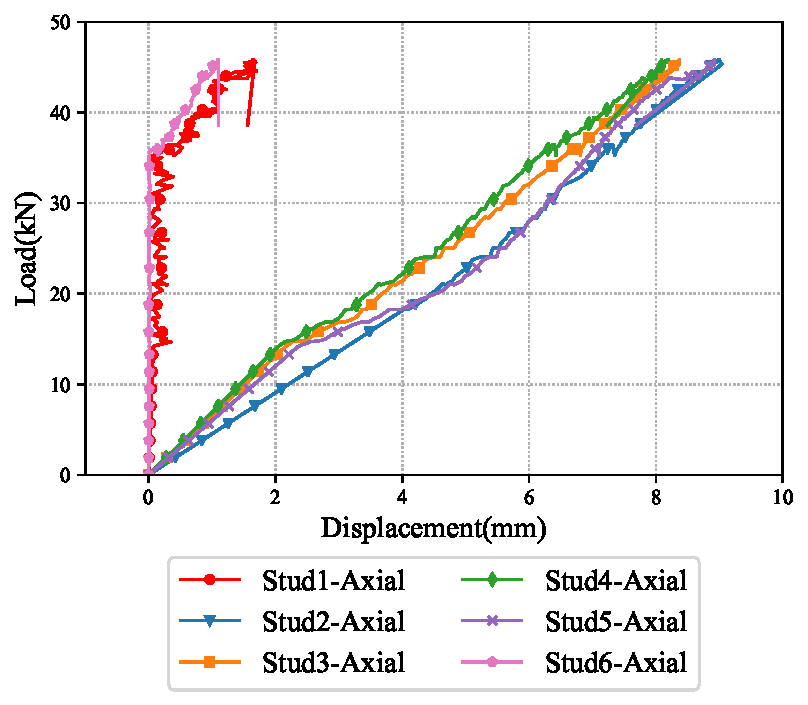
\includegraphics[width=6.5cm,height=6cm]{AT3-Load-Axial-Corrected.pdf} & 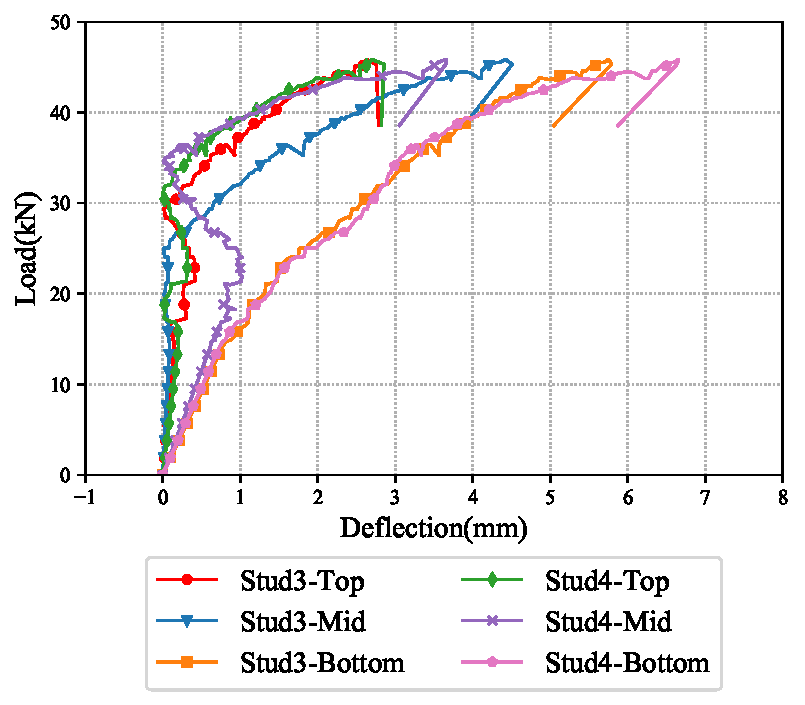
\includegraphics[width=6.5cm,height=6cm]{AT3-Load-Lateral-Corrected.pdf} \\ 
			(a) & (b)  \\ 
		\end{tabular} 
		\caption{Test-AT3 results - (a) Axial displacement and (b) Lateral deflection versus applied axial load}
		\label{fig:AT3-results}
\end{figure}

\section{Ambient Test-AT4}

The ambient Test-T4 was conducted on double stud LSF wall with 70 mm stud depth. The stud dimensions were 70\(\times\)29.5\(\times\)8\(\times\)0.95 mm. This test was conducted to investigate the ambient load carrying capacity of double stud LSF walls with 70 mm studs. Four studs were used for the ambient capacity test and the test configuration is show in \Cref{fig:AT4-plan}. After the initial preloading sequence, axial load was applied in increments to determine the axial compression capacity of the test wall. The test wall resulted in an axial compression load of 86.21 kN at the end of the test. Significant local buckling in Stud3 web and flanges was observed in the test wall post test observation as shown in \Cref{fig:AT4-failure}~(b). The buckling failure was noticeable on one Stud3 in row one only. A large crack on the ambient side plasterboard was also observed at the stud failure location as shown in \Cref{fig:AT4-failure}~(a).
\begin{figure}[!htbp]
	\centering
			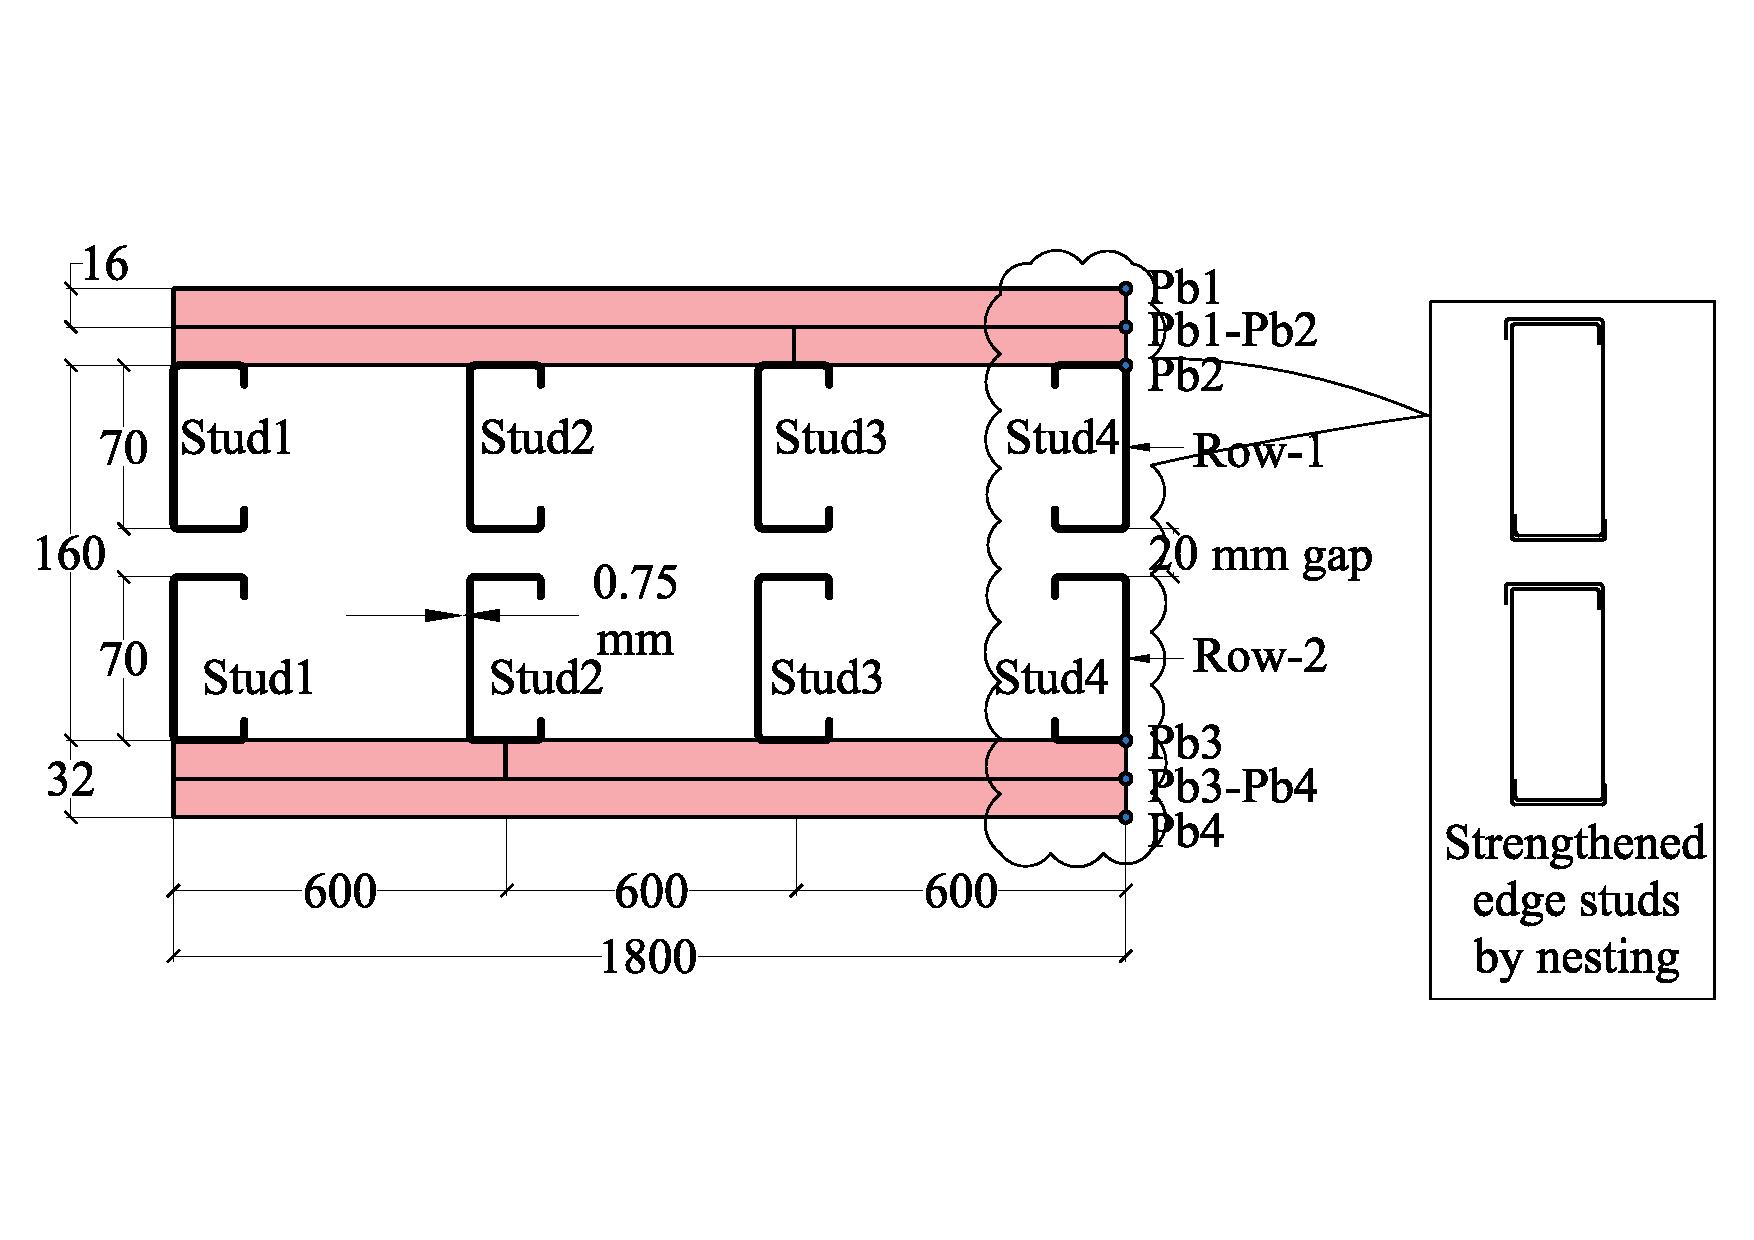
\includegraphics[scale=0.25]{AT4-plan.pdf}\\
		\caption{Test-AT4 configuration}
		\label{fig:AT4-plan}
\end{figure}  
\begin{figure}[!htbp]
	\centering
		\begin{tabular}{cc}
			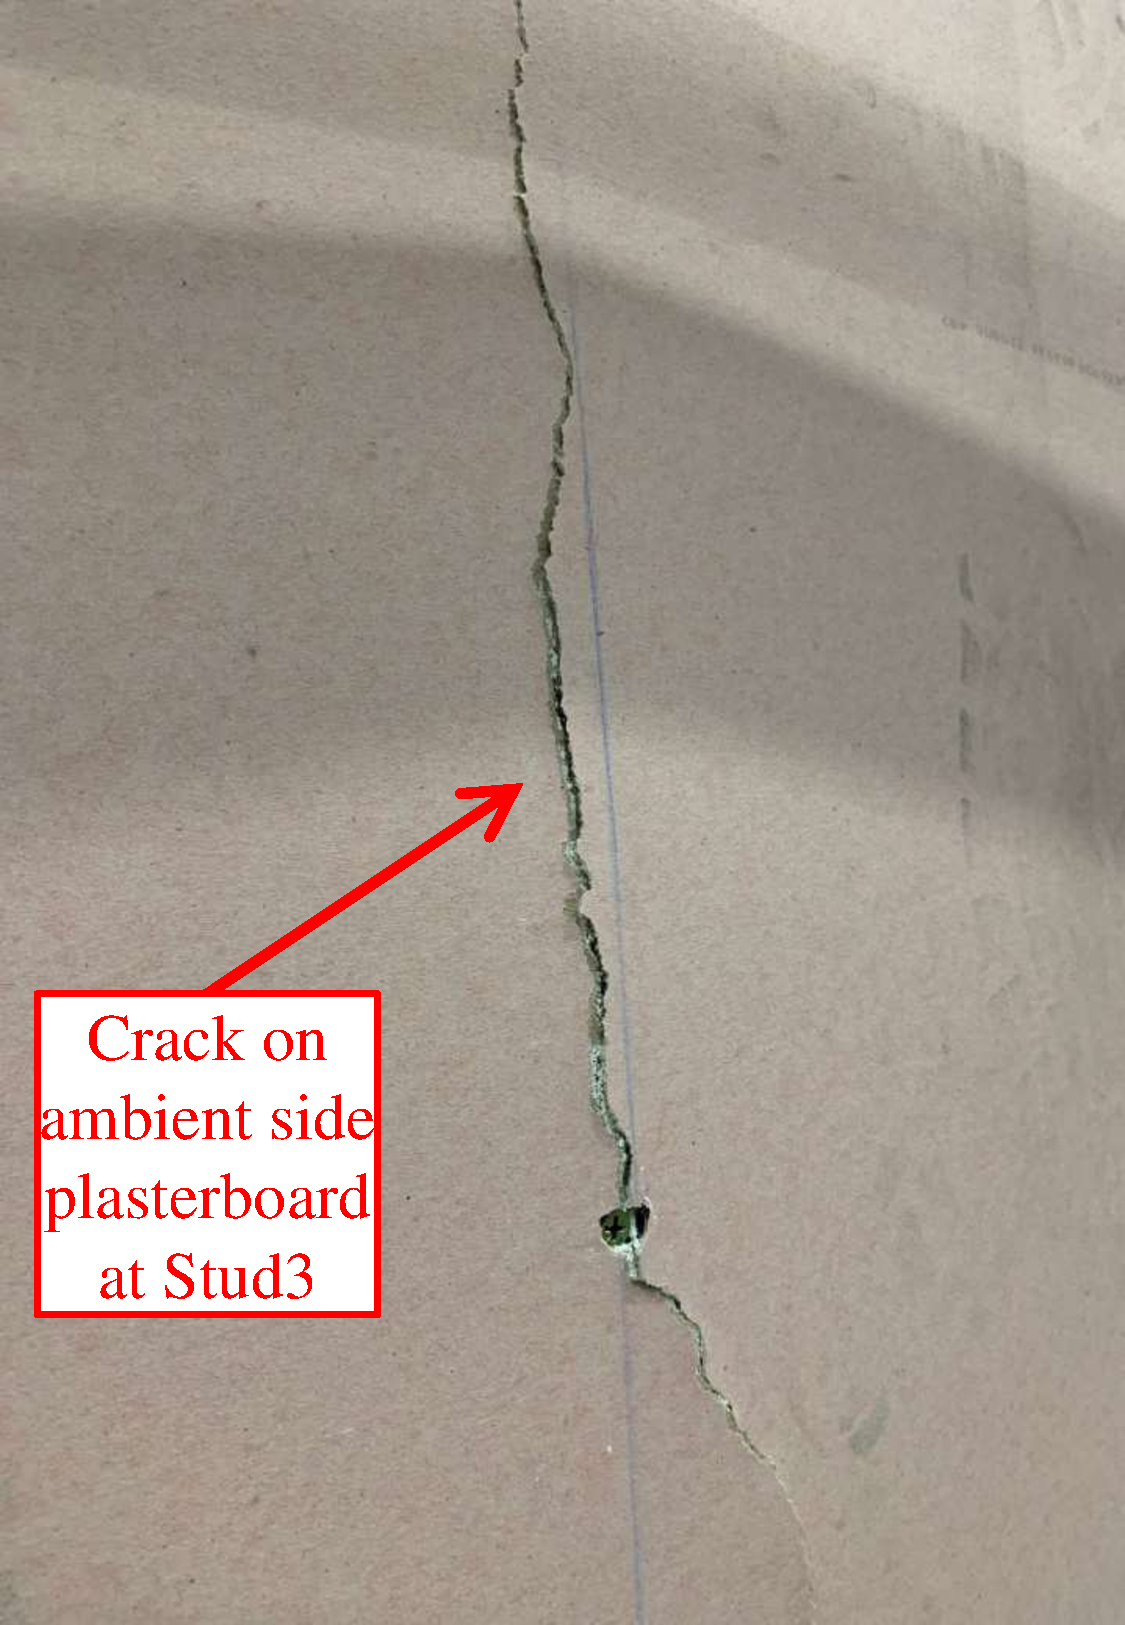
\includegraphics[scale=0.2]{AT4-plasterboard_crack.pdf} & 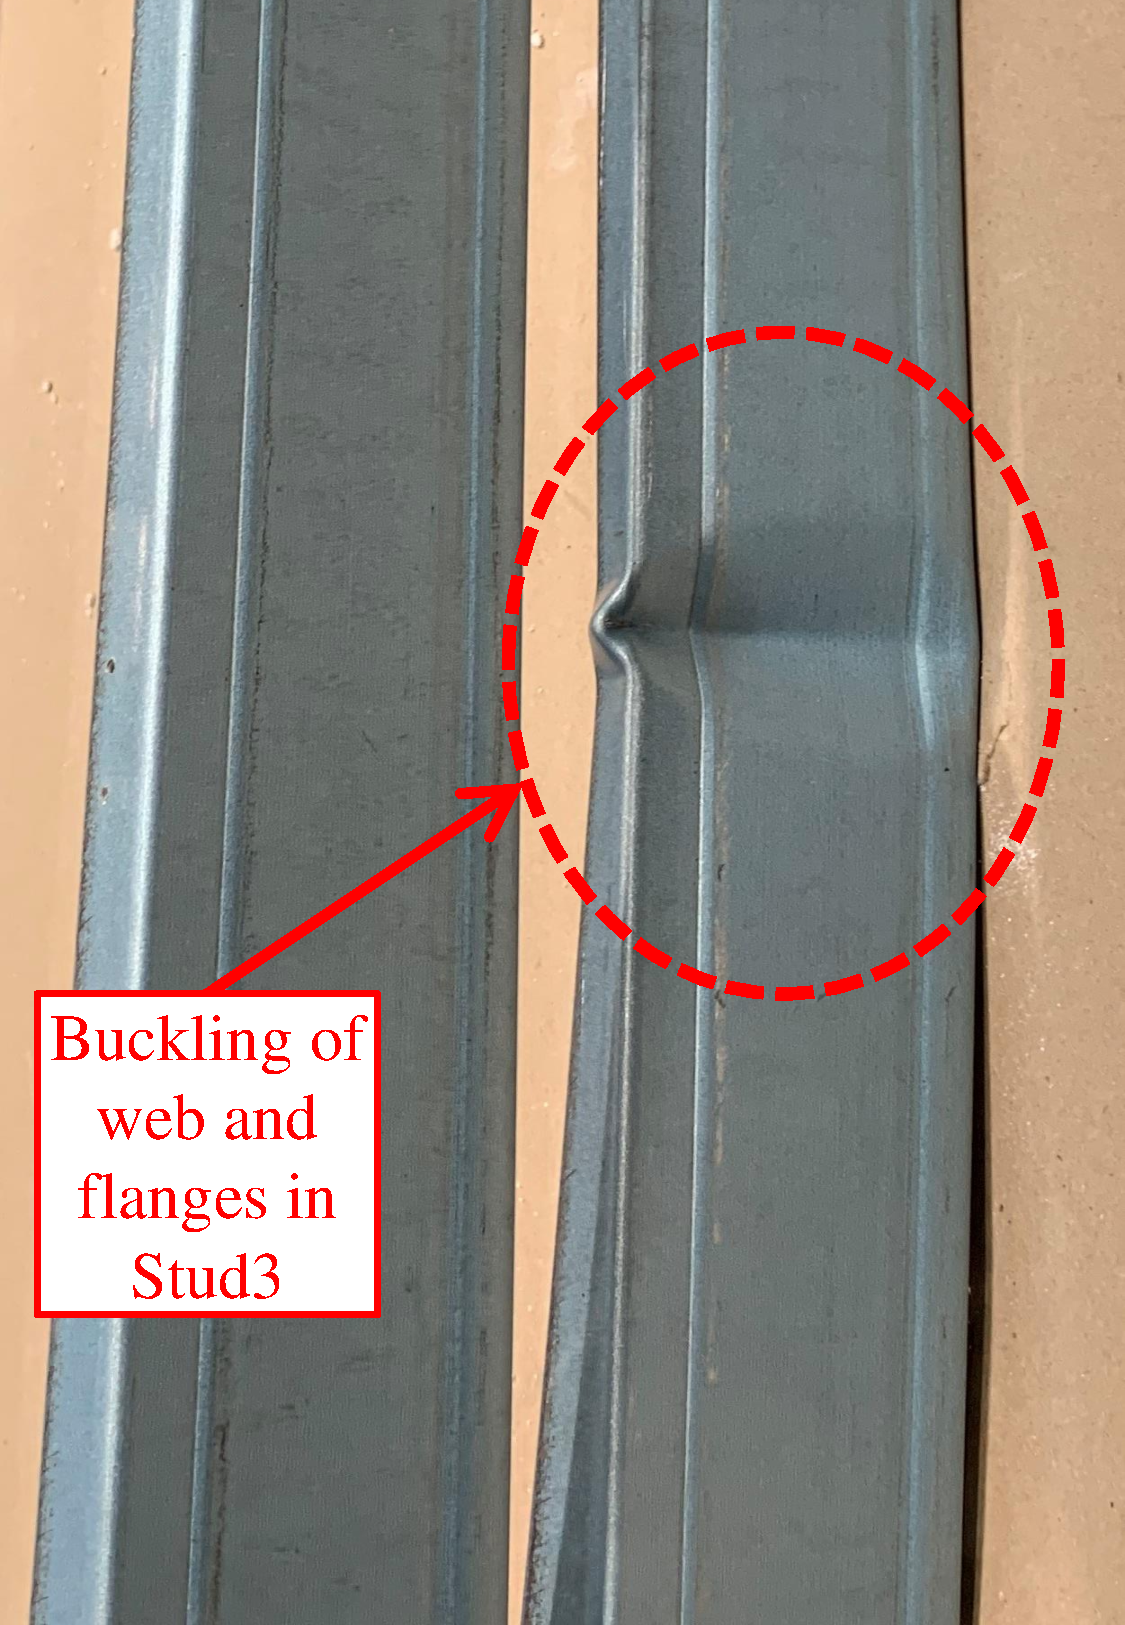
\includegraphics[scale=0.2]{AT4-buckling.pdf} \\ 
			(a) & (b)  \\ 
		\end{tabular} 
		\caption{Test-AT4 results - (a) Plasterboard crack and (b) Buckling of stud}
		\label{fig:AT4-failure}
\end{figure}

The axial displacement and lateral deflection curves of Test-AT4 are shown in \Cref{fig:AT4-results} (a)~and~(b). Maximum axial compression of 31.65 mm was recorded at the LVDT measured at Stud3. This indicates the structural failure on Stud3 as witnessed in \Cref{fig:AT4-failure}~(b). The maximum lateral deflection was 16.77 mm at Stud2-Mid (1500 mm) indicating the out-of plane deflection in the test wall. Comparison with the ambient capacity Test-T1 revealed that the axial compression capacity resulted as a part of this test was higher in comparison with the former. This increase in axial compression capacity has been attributed by several factors such as the geometric dimensions of the studs used in Test-T4. Also, the slenderness ratio (b/t) of the studs used in Test-T1 is 93.68 while it is 71.57 for Test-T3 if the local buckling of the web is considered. Based on the aforesaid criteria the studs used in Test-T1 are more slender in comparison with Test-T4 resulting in an increased axial compression capacity in Test-T3. 
\begin{figure}
	\centering
		\begin{tabular}{cc}
			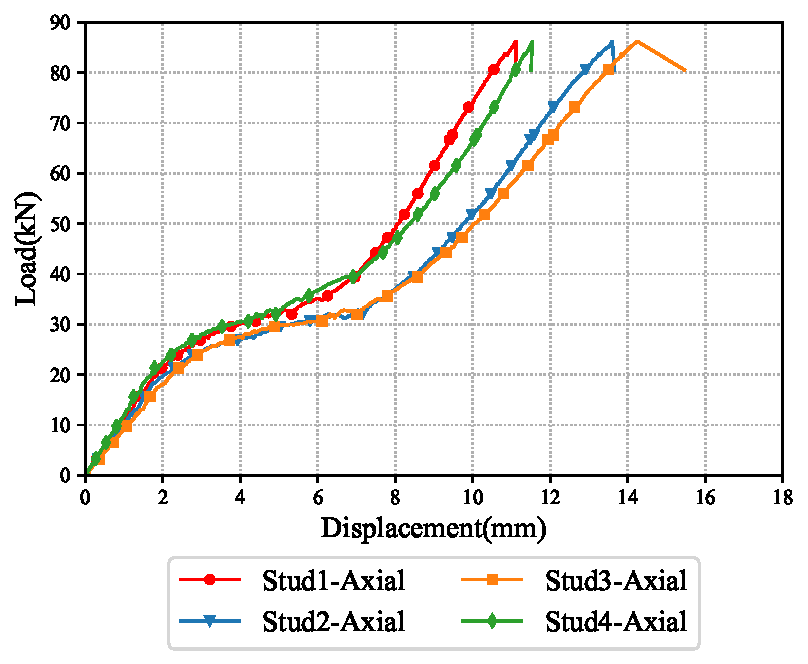
\includegraphics[width=6.5cm,height=6cm]{AT4-Load-Axial-Corrected.pdf} & 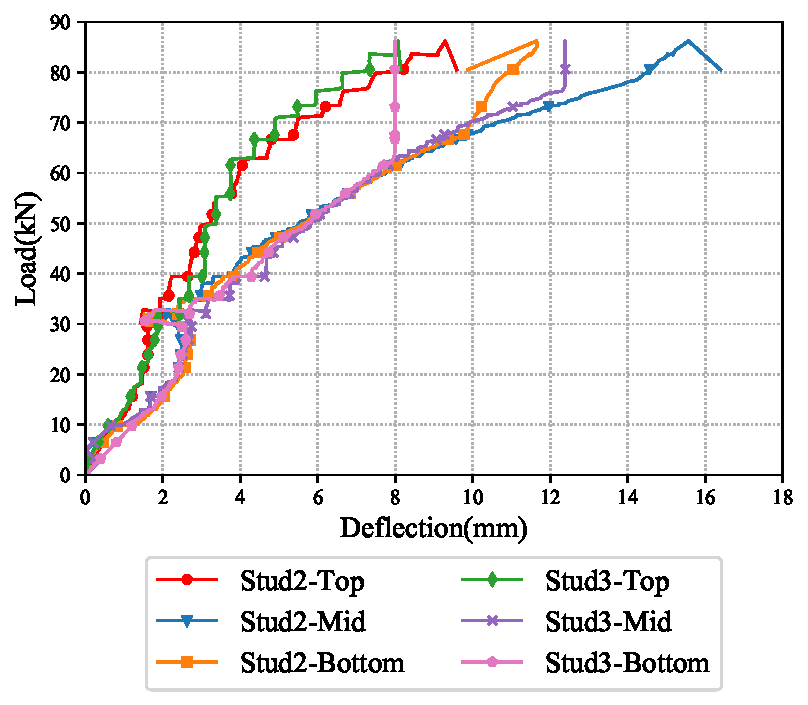
\includegraphics[width=6.5cm,height=6cm]{AT4-Load-Lateral-Corrected.pdf} \\ 
			(a) & (b)  \\ 
		\end{tabular} 
		\caption{Test-AT4 results - (a) Axial displacement and (b) Lateral deflection versus applied axial load}
		\label{fig:AT4-results}
\end{figure}

\section{Ambient Test-AT5}

The last ambient capacity test in the test series was conducted on a staggered stud LSF wall. The configuration of the wall used in this test is distinctive in comparison with other ambient tests. The test wall consisted of two rows of studs positioned in a staggered manner. LCS were used as studs with dimensions measuring 90\(\times\)36\(\times\)7\(\times\)0.95 mm. Total of eleven studs were used in a staggered configuration as shown in \Cref{fig:AT5-plan}. All the ambient capacity tests (AT1-AT4) had UCS noggings connecting the flanges and provide in-plane lateral restraint at 1 m intervals. However, in staggered stud wall the discontinuity between the stud rows are necessary to achieve the required acoustic rating. Therefore, omega noggings were used at 1 m intervals to provide in-plane lateral restraints to the studs under axial compression. The omega noggings are connected to every alternate studs on the stud webs at service holes through a connecting clip. The clips are held on to web at one end and snapped on to the groves of the omega nogging at two locations. The nogging to stud connection details are shown in \Cref{fig:AT5-construction}~(a). End cleats were used to connect the unrestrained stud flanges to the track to facilitate fixity conditions in the ambient capacity test as shown in \Cref{fig:AT5-construction}~(b). 
\begin{figure}[!htbp]
	\centering
			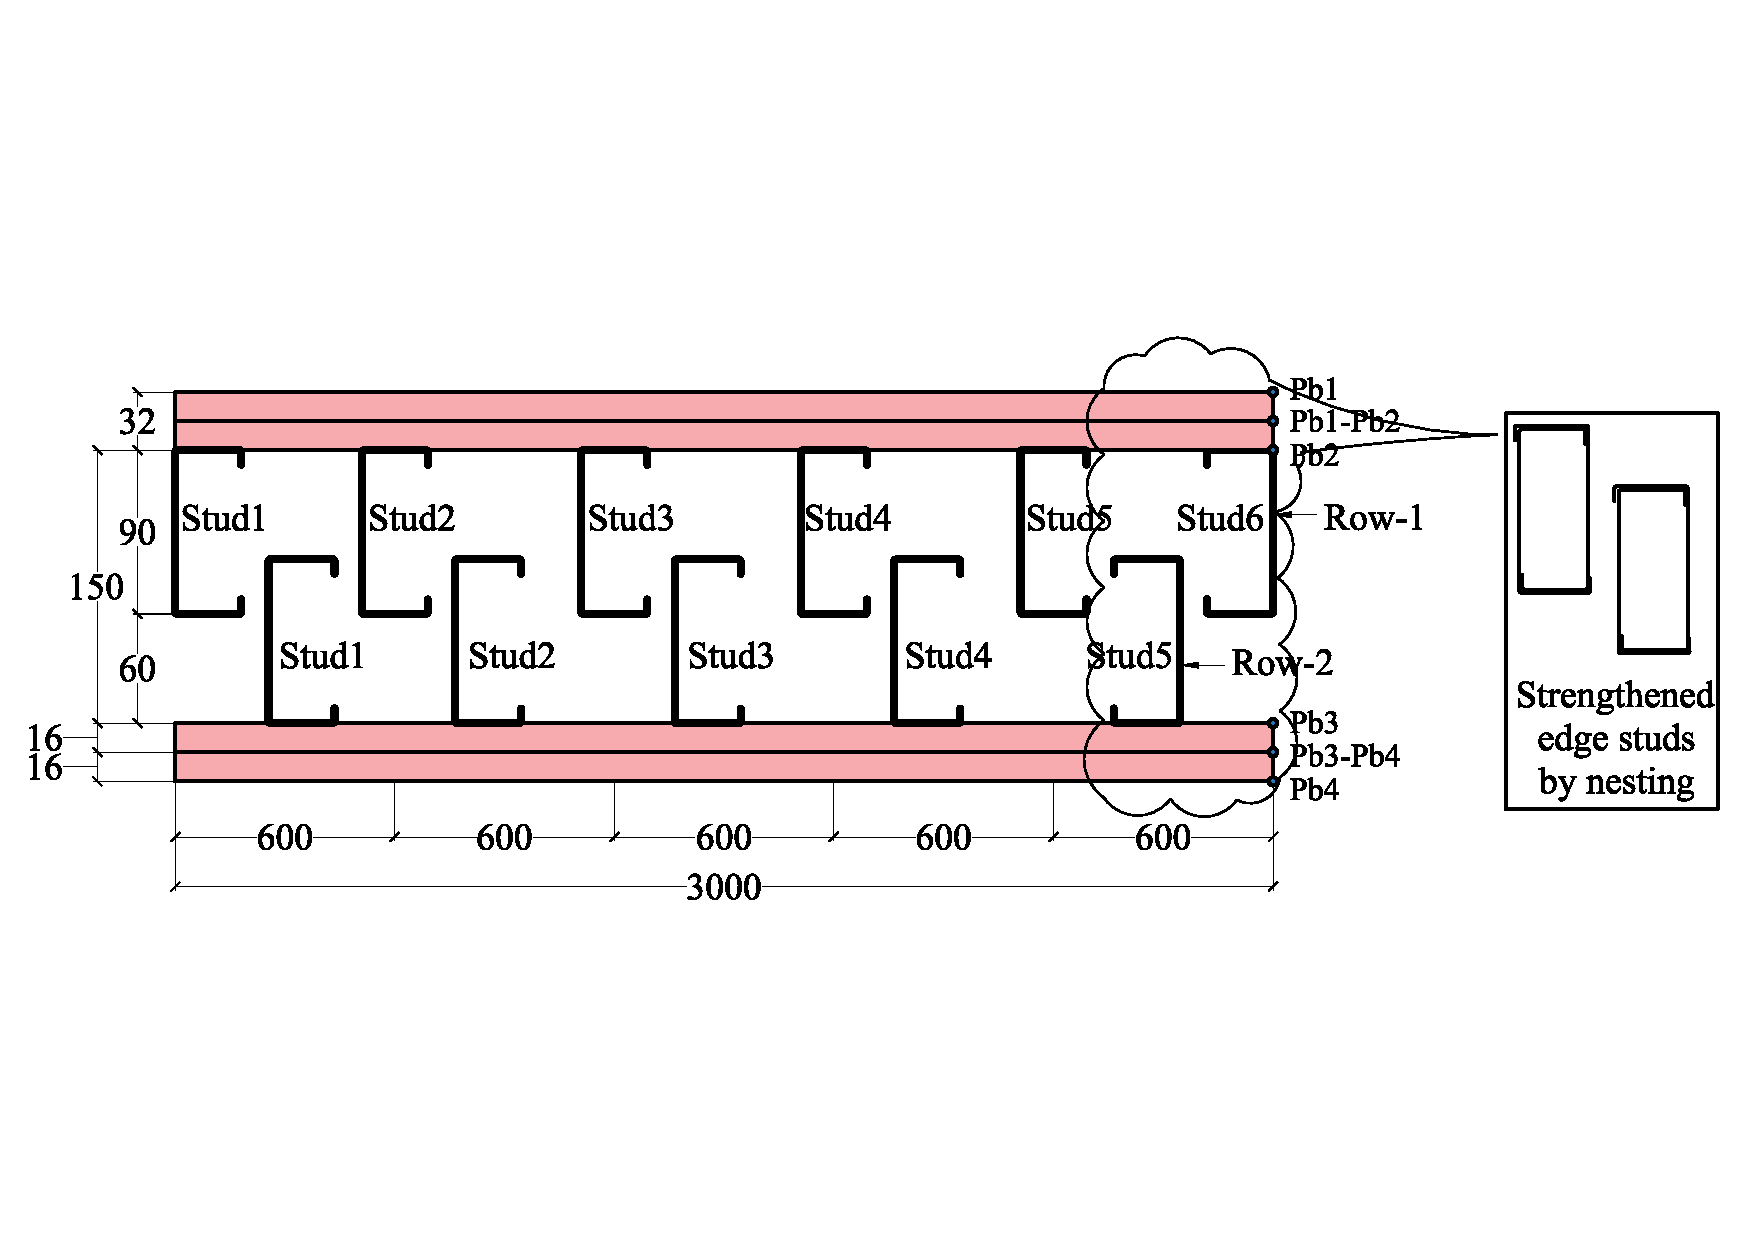
\includegraphics[scale=0.25]{AT5-plan.pdf}\\
		\caption{Test-AT5 configuration}
		\label{fig:AT5-plan}
\end{figure}
\begin{figure}[!htbp]
	\centering
		\begin{tabular}{cc}
			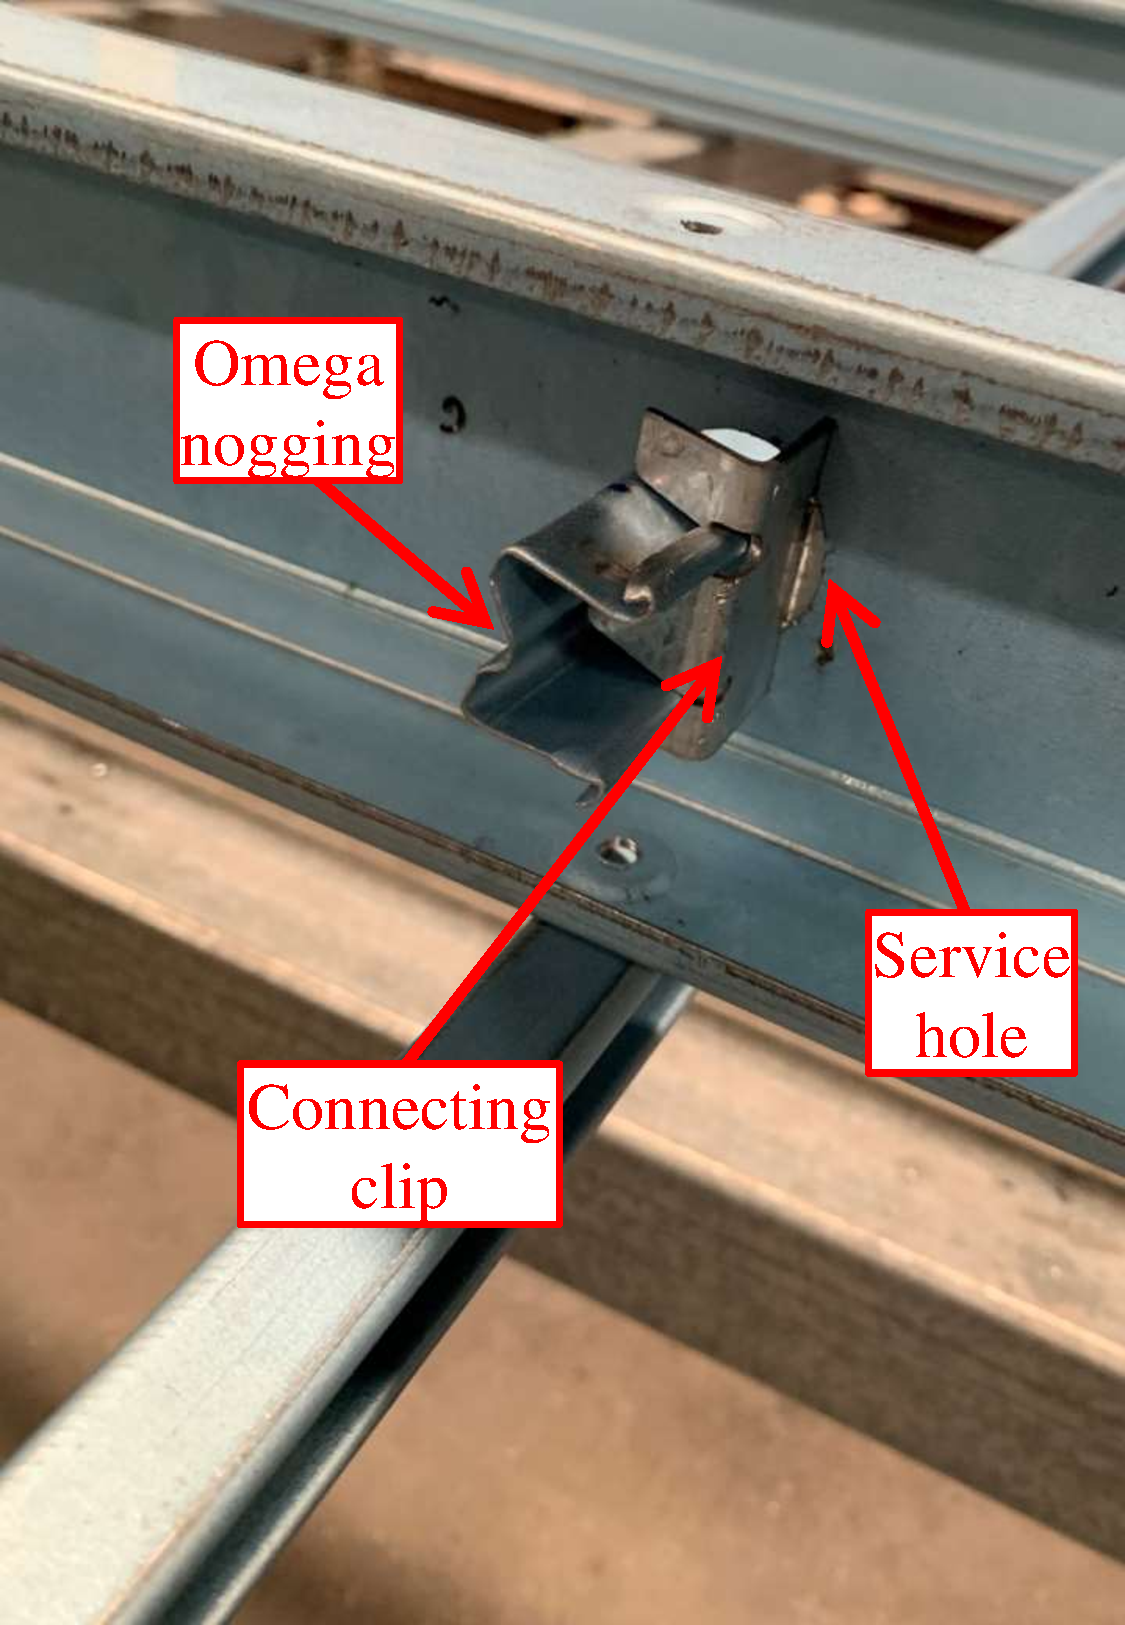
\includegraphics[width=4cm,height=5.5cm]{omega_connection.pdf} & 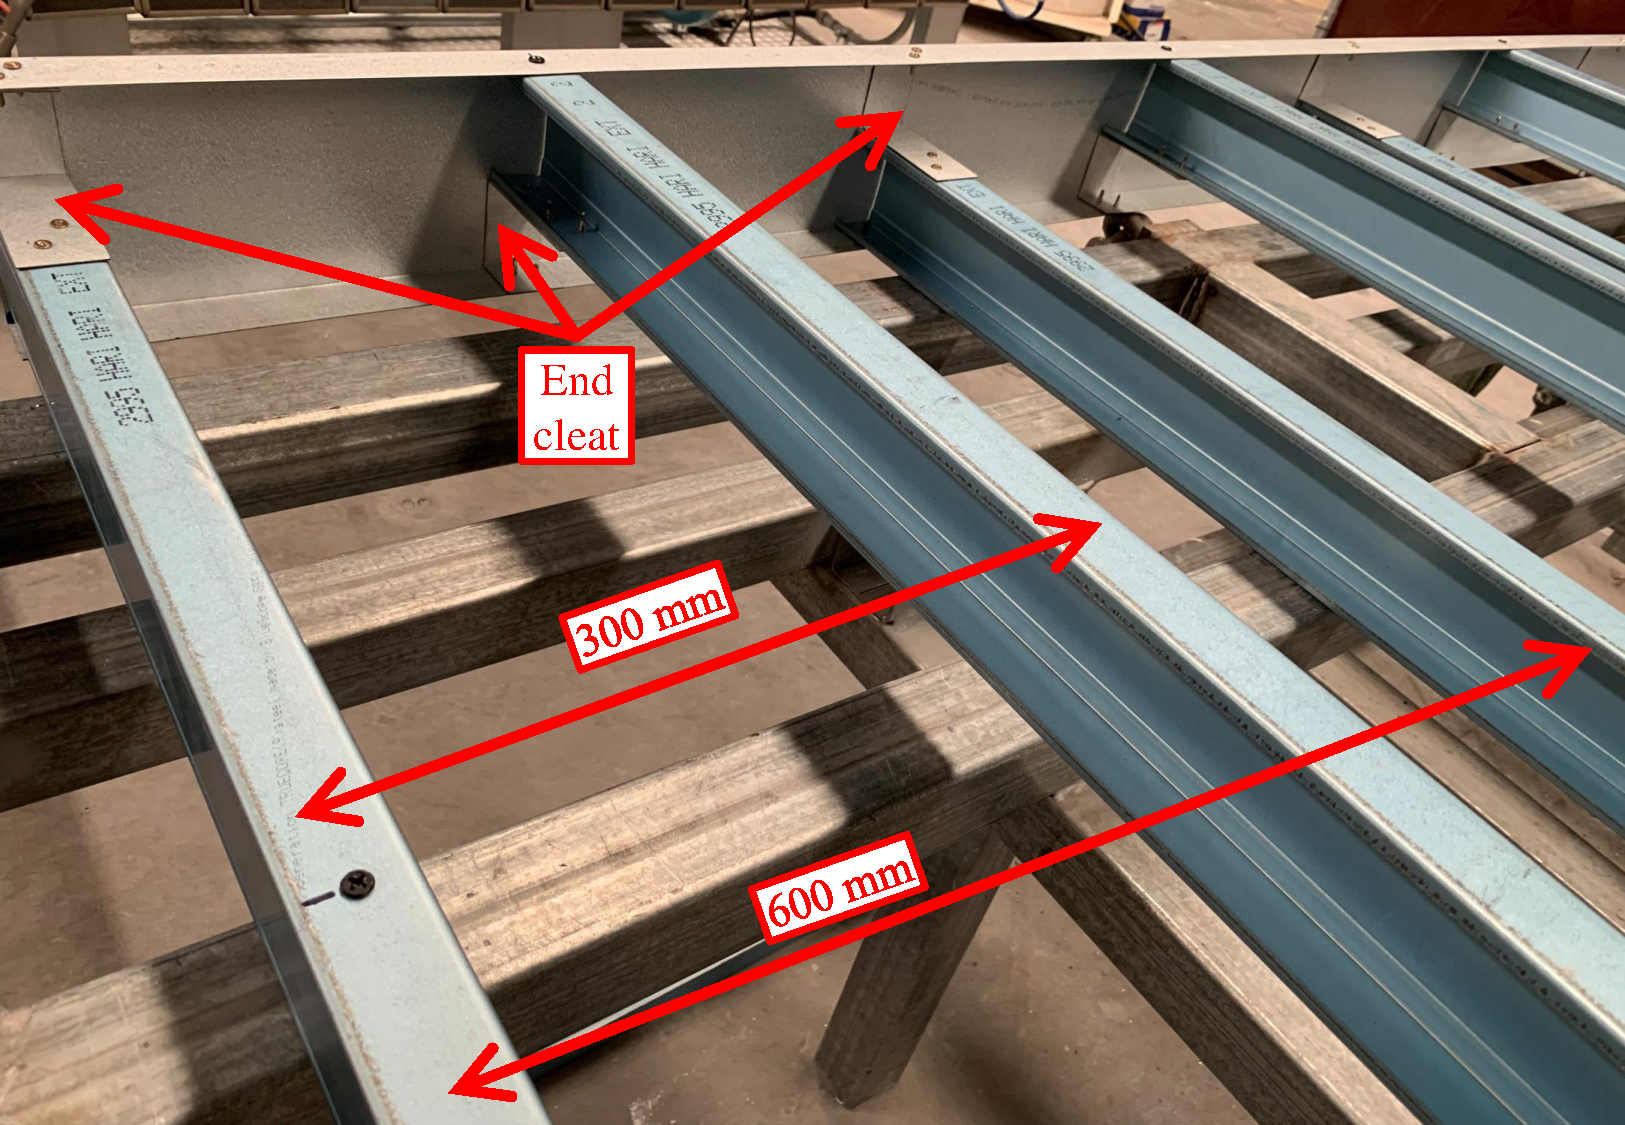
\includegraphics[width=8cm,height=5.5cm]{AT5-construction.pdf} \\ 
			(a) & (b)  \\ 
		\end{tabular} 
		\caption{Test-AT5 - (a) Omega nogging and clip connection (b) Staggered stud wall construction}
		\label{fig:AT5-construction}
\end{figure}
\begin{figure}[!htbp]
	\centering
		\begin{tabular}{cc}
			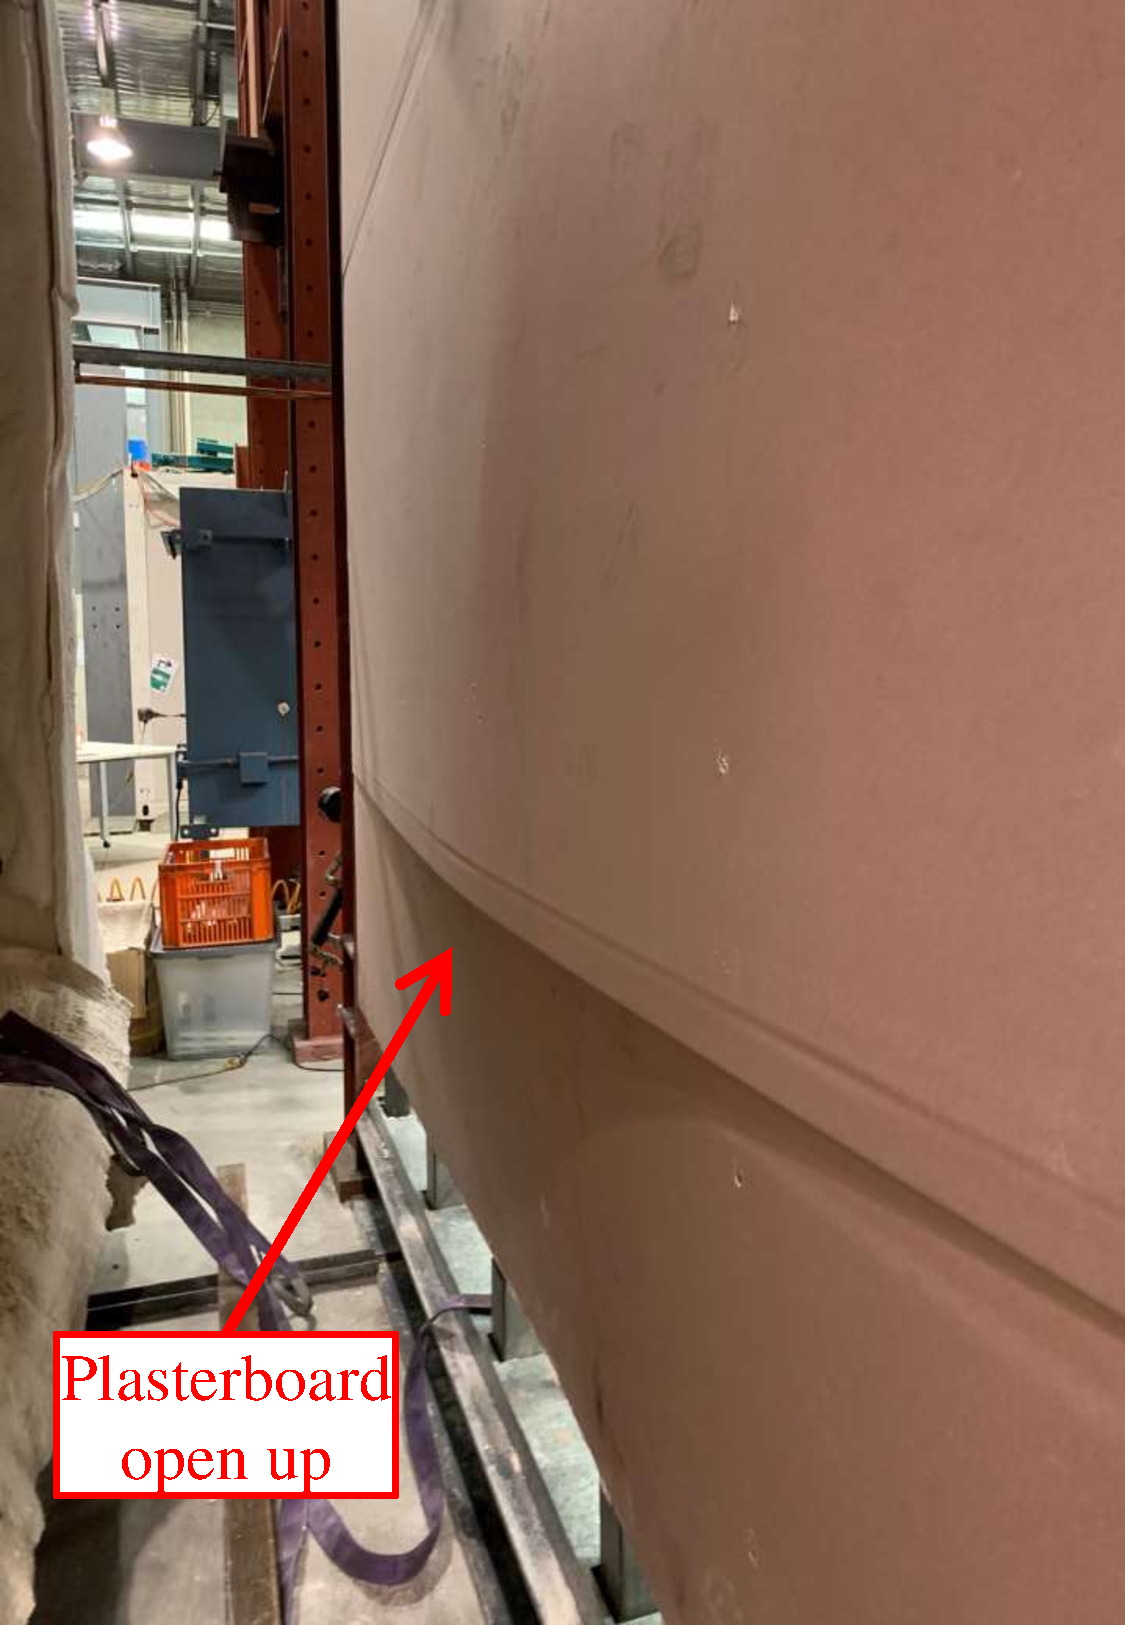
\includegraphics[width=5.5cm,height=8cm]{AT5-plasterboard.pdf} & 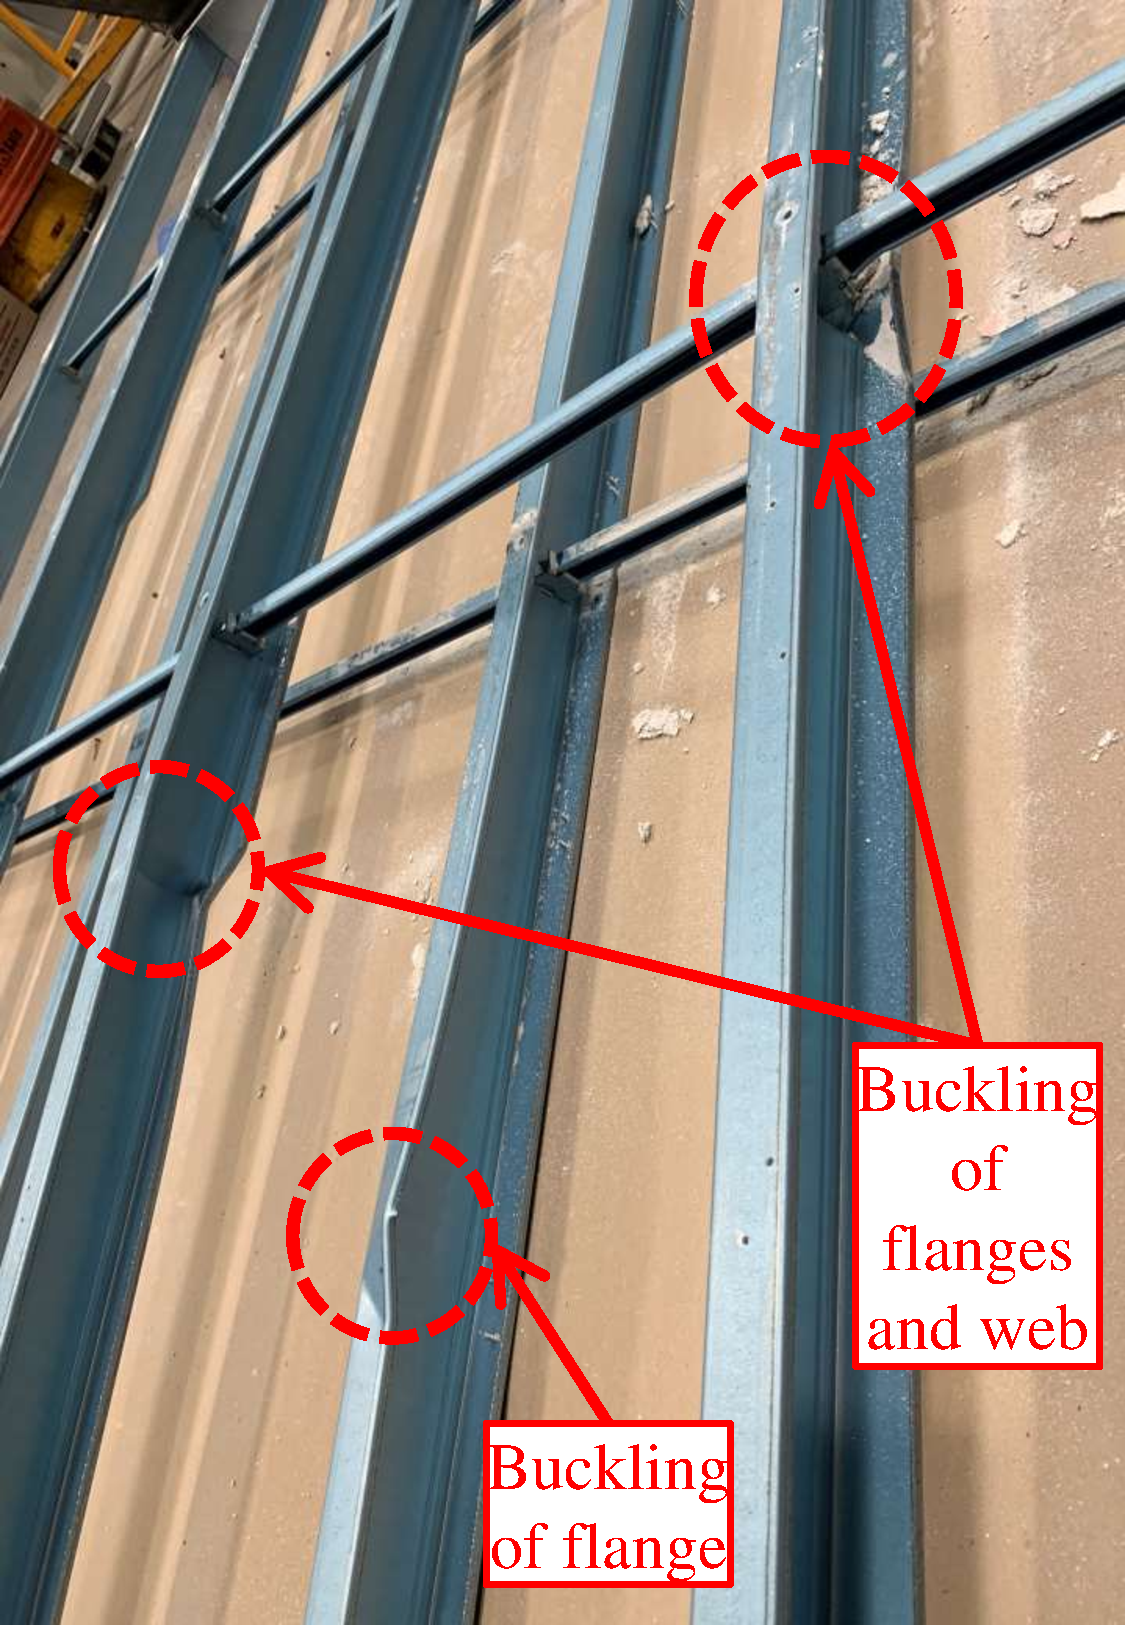
\includegraphics[width=5.5cm,height=8cm]{AT5-buckling.pdf} \\ 
			(a) & (b)  \\ 
		\end{tabular} 
		\caption{Test-AT5 - failure (a) Plasterboard open up and (b) Buckling of studs}
		\label{fig:AT5-failure}
\end{figure}
\begin{figure}
	\centering
		\begin{tabular}{cc}
			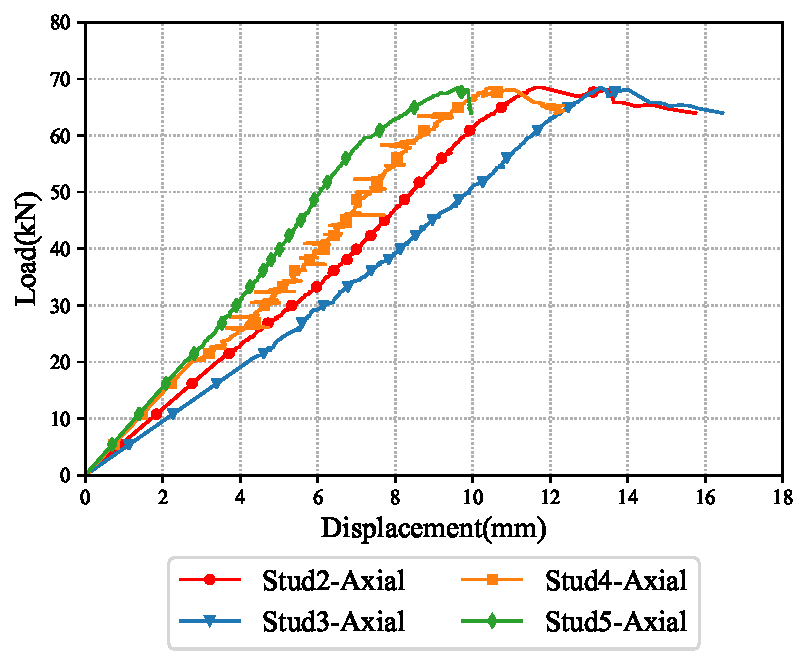
\includegraphics[width=6.5cm,height=6cm]{AT5-Load-Axial-Corrected.pdf} & 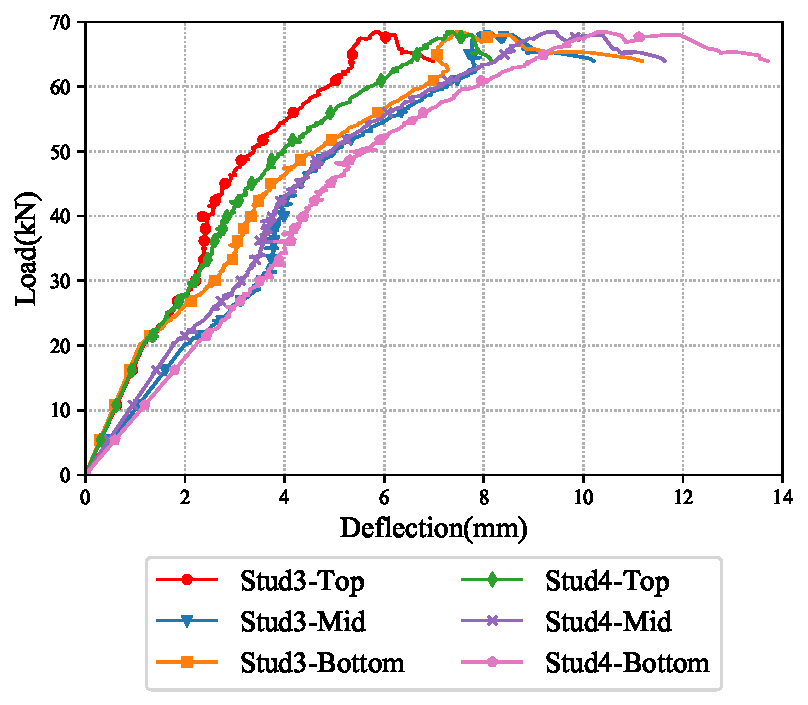
\includegraphics[width=6.5cm,height=6cm]{AT5-Load-Lateral-Corrected.pdf} \\ 
			(a) & (b)  \\ 
		\end{tabular} 
		\caption{Test-AT5 results - (a) Axial displacement and (b) Lateral deflection versus applied axial load}
		\label{fig:AT4-results}
\end{figure}

The test wall was loaded through a 20 mm thick base plate connecting the rams and the axial compression load was applied individually to the staggered studs. The end studs of the test wall were strengthened as the plasterboards do not provide effective lateral restraints to the end studs as discussed in \Cref{sec:AT1}. After the application of initial preload the ambient capacity test was conducted by gradual increase in the applied axial load till failure. The test wall resulted an axial compression capacity of 68.49 kN. A maximum axial displacement of 21.62 mm was recorded in Stud3 at the end of the test. The maximum lateral deflection of 13 mm was recorded at 750 mm from the bottom of the specimen near Stud4. Plasterboard open up was noticeable near the stud failure locations as shown in \Cref{fig:AT5-failure}~(a). Local buckling of the web and flanges were observed post test investigation as shown in \Cref{fig:AT5-failure}~(b).

\section{Summary of Ambient Capacity Tests}

The summary of all the ambient capacity tests conducted on double and staggered stud LSF walls are presented and discussed in this section. A total of five ambient capacity tests were conducted and the results are summarised in the \Cref{tab:ambient-test-results}. The axial compression capacity of 90 mm and 70 mm wide studs with various thicknesses and stud configurations were considered for the investigation. Ambient tests AT1 to AT4 were conducted on double stud walls with 90 mm and 70 mm wide studs. The cavity depth of the test wall was 200 mm for Tests-AT1 to AT3 while it was 160 mm for Test-AT4. Thickness of the studs were 0.95 mm for Tests-AT1 and AT4 while the thickness was 0.75 mm for Test-AT2 and AT3. Test-AT5 was conducted on staggered stud LSF wall comprising of 90 mm studs with a cavity depth of 150 mm and a stud thickness of 0.95 mm.  
\begin{table}[!htbp]
	\centering
	\caption{Ambient test panel details - Summary}
	\begin{tabular}{ccccccc}
		\toprule
		\multicolumn{1}{m{2.4em}}{\centering{Test Name}} & 
		\multicolumn{1}{m{5.6em}}{\centering{Description}} & 
		\multicolumn{1}{m{2.85em}}{\centering{Stud Depth (mm)}} & 
		\multicolumn{1}{m{2.85em}}{\centering{Cavity Depth (mm)}} & 
		\multicolumn{1}{m{5em}}{\centering{Stud Thickness (mm)}} & 
		\multicolumn{1}{m{3em}}{\centering{No of Studs}} &
		\multicolumn{1}{m{3em}}{\centering{Failure Load (kN)}} \\
		\midrule
		AT1  & Double Stud & 90 & 200 & 0.95 & 4 & 73 \\
		AT2  & Double Stud & 90 & 200 & 0.75 & 4 & 47.08 \\
		AT3  & Double Stud & 90 & 200 & 0.75 & 6 & 39.42 \\
		AT4  & Double Stud & 70 & 160 & 0.95 & 4 & 86.21 \\
		AT5  & Staggered Stud & 90 & 200 & 0.95 & 6 & 68.49 \\
		\bottomrule
	\end{tabular}%
	\label{tab:ambient-test-results}%
\end{table}%

The double stud wall Test-AT1 with 0.95 mm thick 90 mm wide studs resulted in an axial compression capacity of 73 kN while Test-AT4 which had the same stud thickness and 70 mm wide studs resulted in an axial compression capacity of 86 kN. This is 13 kN higher in comparison with Test-AT1. The reduction in axial compression capacity is attributed by the higher slenderness ratio of the studs in Test-AT1 due to the geometric profile. The Tests-AT2 and AT3 resulted in an axial compression capacity of 47.08 and 39.42 kN. Despite the same testing configuration and stud thickness the number of studs were only varied. The variation in axial compression capacity was due to the absence of effective plasterboard restraints to the end studs resulting in bearing failure at supports. However, the difference in axial compression capacity between the Tests-AT2 and AT is small and can be ignored. The staggered stud wall Test-AT5 resulted in an axial compression capacity of 68.49 kN which is comparatively closer to Test-AT1 with the same stud depth and thickness. However, the arrangement of studs were different in both the tests. In Test-T1 the test wall had the stud rows in a linear pattern while in Test-T5 the studs were staggered. The effective centre-to-centre distance between the studs were 600 mm in the double stud wall Test-T1 while it was 300 mm in the staggered stud wall Test-AT5. But it is to note that the cavity depth of Test-AT1 was 200 mm while it was 150 mm for Test-AT5 which is beneficial in reducing effective floor space in LSF wall construction.

\section{Comparison of Ambient Capacity Test Results}

As the ambient capacity tests were conducted for two different configurations, it becomes a necessity to compare the test results to determine a better understanding about the axial compression behaviour of these complex LSF walls under ambient conditions. Also Test-T1 to T4 were conducted using LCS noggings while Test-T5 was conducted with omega noggings. This adds to the novelty of the ambient capacity tests. The stud flanges in single stud walls are effectively restrained by plasterboard on both sides while in complex LSF walls the effective restraints provided by the plasterboard is limited to one flange only. Therefore, comparisons are made against ambient capacity test results from single stud wall with 92 mm studs and 150 mm studs to understand the difference in axial compression behaviour of the complex LSF walls. Test results used for the comparison are detailed in \Cref{tab:ambient-test-results-comparison}. Comparisons with the 90 mm single stud are made against tow thicknesses 0.75 and 1.15, while for 150 mm single studs the comparisons are made against 1.15 mm thickness only. This is due to the limited availability of the ambient capacity test results. Single stud tests were conducted previously at QUT Wind and Fire Engineering Laboratory. Further details about Test-S-AT2 can be found in \citet{Gunalan2013e}, while for Test-S-T1 and S-T2 details are available as internal reports. 
\begin{table}[!htbp]
	\centering
	\caption{Ambient test panel details - Summary}
	\begin{tabular}{ccccccc}
		\toprule
		\multicolumn{1}{m{2.4em}}{\centering{Test Name}} & 
		\multicolumn{1}{m{5.6em}}{\centering{Description}} & 
		\multicolumn{1}{m{2.85em}}{\centering{Stud Depth (mm)}} & 
		\multicolumn{1}{m{2.85em}}{\centering{Cavity Depth (mm)}} & 
		\multicolumn{1}{m{5em}}{\centering{Stud Thickness (mm)}} & 
		\multicolumn{1}{m{3em}}{\centering{No of Studs}} &
		\multicolumn{1}{m{3em}}{\centering{Failure Load (kN)}} \\
		\midrule
		AT1  & Double Stud & 90 & 200 & 0.95 & 4 & 73 \\
		AT2  & Double Stud & 90 & 200 & 0.75 & 4 & 47.08 \\
		AT4  & Double Stud & 70 & 160 & 0.95 & 4 & 86.21 \\
		AT5  & Staggered Stud & 90 & 150 & 0.95 & 11 & 68.49 \\
		S-AT1 & Single Stud & 90 & 90 & 0.75 & 2 & 33.10 \\
		S-AT2 & Single Stud & 90 & 90 & 1.15 & 4 & 79.24 \\
		S-AT3 & Single Stud & 150 & 150 & 1.15 & 6 & 45.43 \\
		\bottomrule
	\end{tabular}%
	\label{tab:ambient-test-results-comparison}%
\end{table}%

Firstly comparisons were made against 90 mm studs on single and double stud LSF walls. This include stud thickness of 0.75, 0.95 and 1.15 mm. Secondly, comparisons were made against staggered stud and single stud wall with 150 mm cavity depth. The stud thickness used in staggered stud wall was 0.95 mm with 90 mm stud depth while for single stud wall 150 mm deep studs with 1.15 mm thickness were used. Also, the 70 mm stud double stud wall Test-AT4 was also compared to understand the axial compression capacity of the single and double stud walls under different plasterboard restraint conditions. Comparisons are made against the maximum axial load carrying capacity. Variations in effective restraints provided by plasterboards for different configurations are also discussed and their effect on the axial load carrying capacity was also investigated. Applied load versus axial displacement is compared against single and double stud walls with 90 and 150 mm cavity depth and are shown in \Cref{fig:90mm-comparison-ambient,fig:150mm-comparison-ambient}.
\begin{figure}[!htbp]
	\centering
			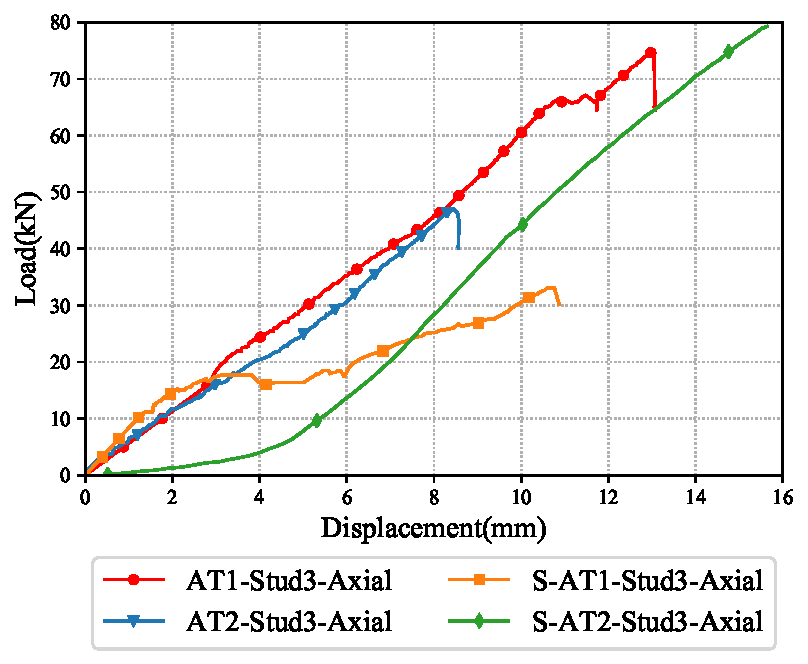
\includegraphics[width=10cm,height=9cm]{90mm-Axial-comparison.pdf}\\
		\caption{Tensile coupon details}
		\label{fig:90mm-comparison-ambient}
\end{figure}
\begin{figure}[!htbp]
	\centering
			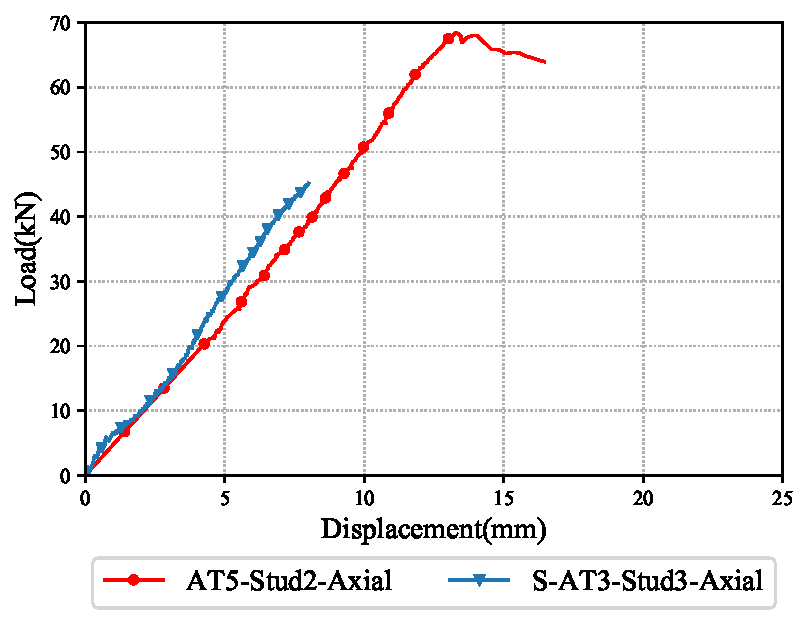
\includegraphics[width=10cm,height=9cm]{150mm-Axial-comparison.pdf}\\
		\caption{Tensile coupon details}
		\label{fig:150mm-comparison-ambient}
\end{figure}

Maximum axial compression capacity was recorded in single stud wall with stud thickness of 1.15 mm (S-AT2) resulting in a failure load of 79.24 kN. The least axial compression capacity was recorded in single stud wall with 0.75 mm stud (S-AT1) resulting in a failure load of 33.10 kN. In single stud LSF walls, the plasterboards provide effective lateral restraints preventing the in plane buckling of studs. As the studs locally buckle, the out of plane plasterboard restraint is not generally critical under ambient conditions. However, in the case of single stud wall with 150 mm studs the axial compression capacity was 45.43 kN which is 33.81 kN lesser than the corresponding single stud wall with 90 mm studs. This is attributed by the wider web depth in 150 mm studs resulting in lesser axial compression capacity.

In case of double stud LSF walls the effective plasterboards restraints are provided to one flange only on each stud rows. The inner stud flanges in the LSF wall are restrained at 1 m intervals through noggings. This results in inadequate in-plane plasterboard restraints to the studs resulting in reduced axial compression capacity. If the double stud wall Test-AT1 is taken for consideration, an axial compression capacity of 73 kN was recorded for both the stud rows. This attributes to 36.5 kN per stud which is 42.74 kN less than single stud wall Test-S-AT1 with 90 mm studs restrained on both the flanges. However, it is to note that the double stud wall was tested with a stud thickness of 0.95 mm while the single stud wall had a stud thickness of 1.15 mm. It can be inferred that the thickness of the studs significantly affect the axial compression capacity under ambient conditions. If the single stud wall Test-S-AT1 is compared with the double stud wall Test-AT2, in which the studs thickness was 0.75 mm in both the cases, the axial compression capacity was 23.54 kN per stud (47.08/2) in double stud wall Test-AT2, whereas it was 33.10 kN in single stud wall Test-S-AT1. The reduction in axial compression capacity was 9.56 kN. However, the double stud wall Test-AT4 with 70 mm studs resulted in a higher axial compression capacity of 86.21 kN (86.21/2 = 43.105 kN per stud) in comparison with double stud wall with 90 mm studs (Test-AT1). Despite having the same stud thickness and wall configuration the 70 mm double stud wall resulted in higher axial compression capacity. This can be attributed to higher slenderness in 90 mm studs in comparison with the 70 mm studs. However, the axial compression capacity of 90 mm single stud LSF wall lined with plasterboard on both sides resulted in a higher compression capacity in comparison with double and staggered stud walls 

Comparing the LSF walls with 150 mm cavity depth, the axial compression capacity was 68.49 kN in staggered stud wall Test-AT5 and 45.43 kN in 150 mm single stud wall Test-S-AT3. This is a significant reduction in the axial compression capacity. It is to note that the stud spacing was staggered with an effective spacing of 300 mm in staggered stud wall Test-AT5 while the stud spacing was maintained at 600 mm in 150 mm wide single stud wall Test-S-AT3. Also, the omega noggings were connected through the stud webs while no nogging restraints were provided for Test-S-AT3. Despite having a higher stud thickness of 1.15 mm the 150 mm wall Test-S-AT3 resulted in a reduced axial compression capacity. 

\section{Tensile Coupon Tests}

Tensile coupon tests were conducted to determine the Young's Modulus and yield strength of the steel studs in LSF wall, later to be used for numerical analysis. Details of the coupon specimen is given in \Cref{fig:tensile-coupon-details}. Coupons were cut on the web and flanges of the studs at three locations along the 3 m long studs to arrive at the weighted average values of yield strength. The tensile coupon tests were conducted using Instron machine which operates on Bluehill software. Extensometers were used to measure the rate of elongation during the test through which corresponding strain was computed. Detail view of specimen used for the tensile coupon test is shown in \Cref{fig:tensile-coupon-details}.  
\begin{figure}[!htbp]
	\centering
			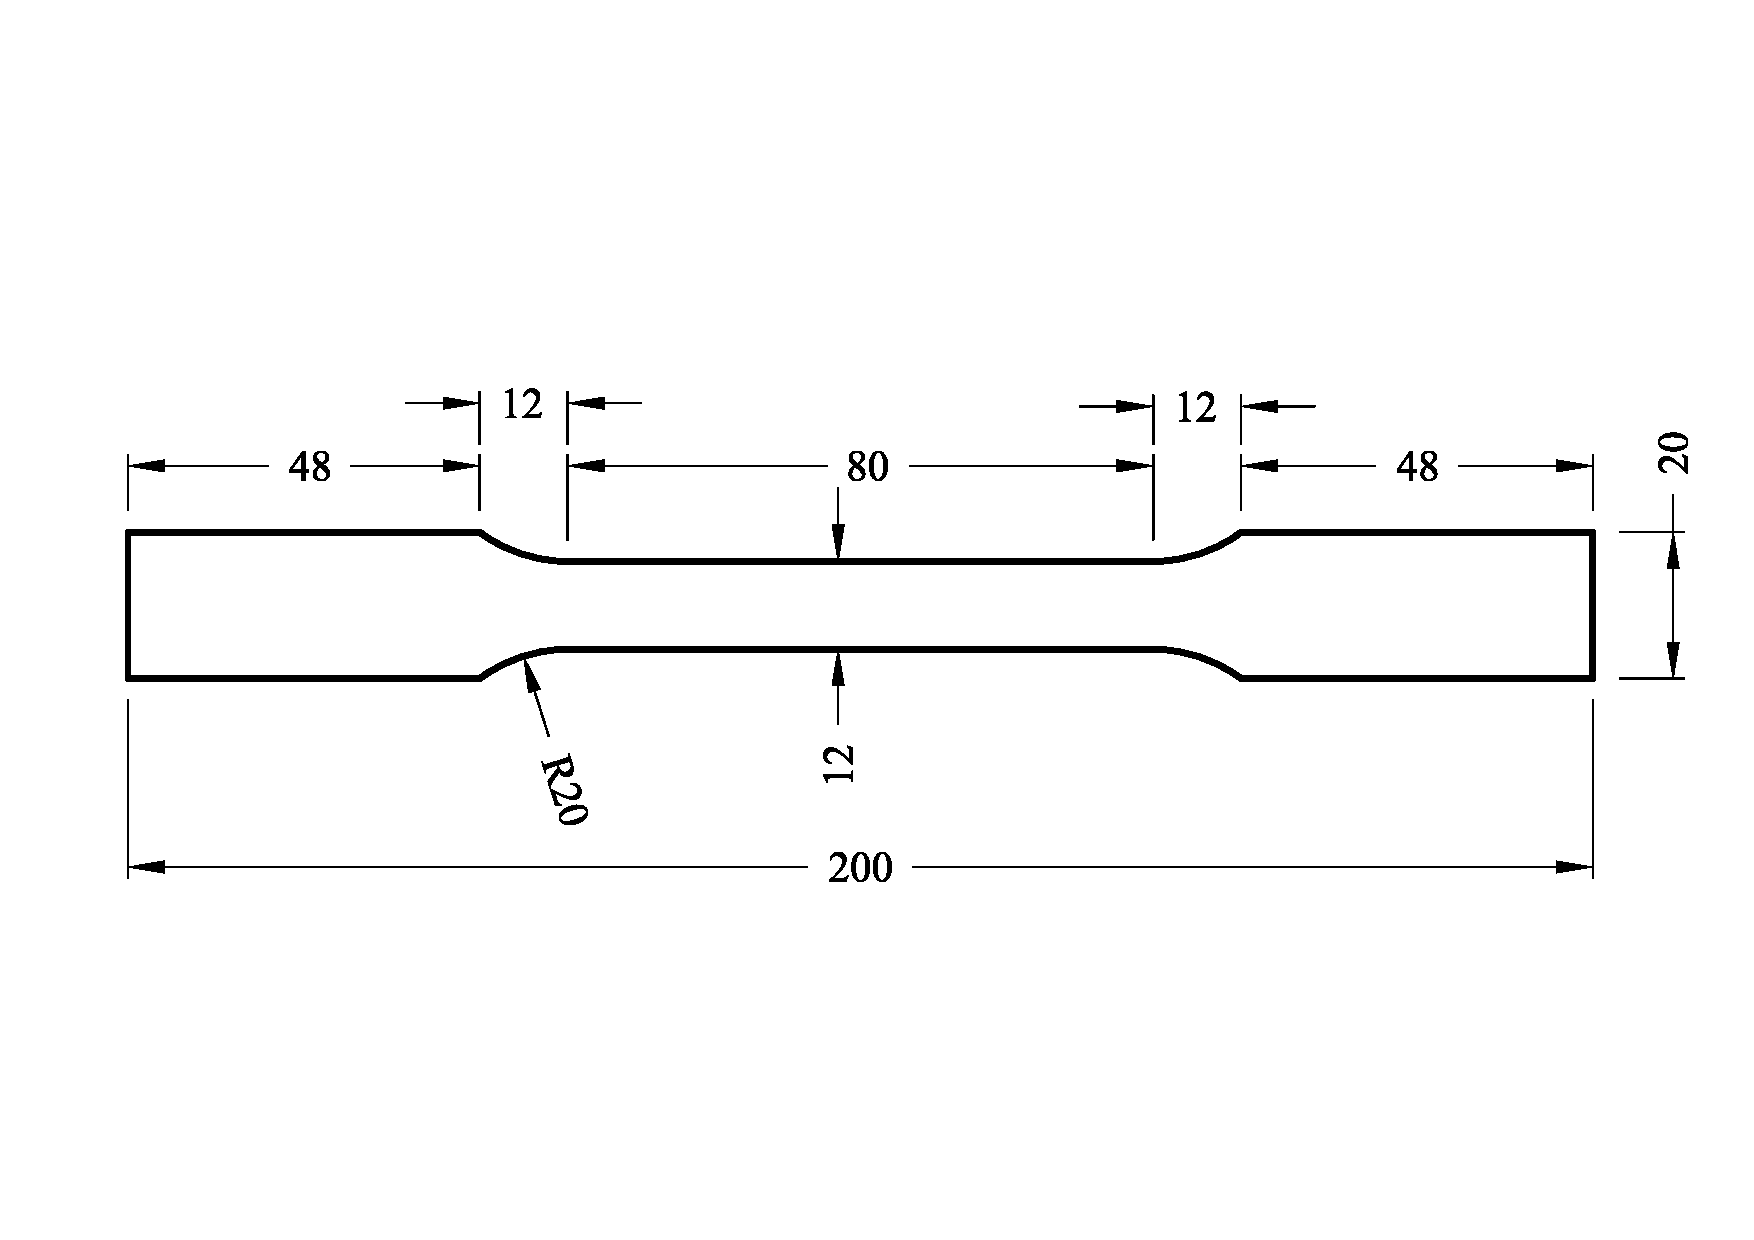
\includegraphics[scale=0.4]{tensile-coupon-details}\\
		\caption{Tensile coupon details}
		\label{fig:tensile-coupon-details}
\end{figure}
\begin{figure}[!htbp]
	\centering
			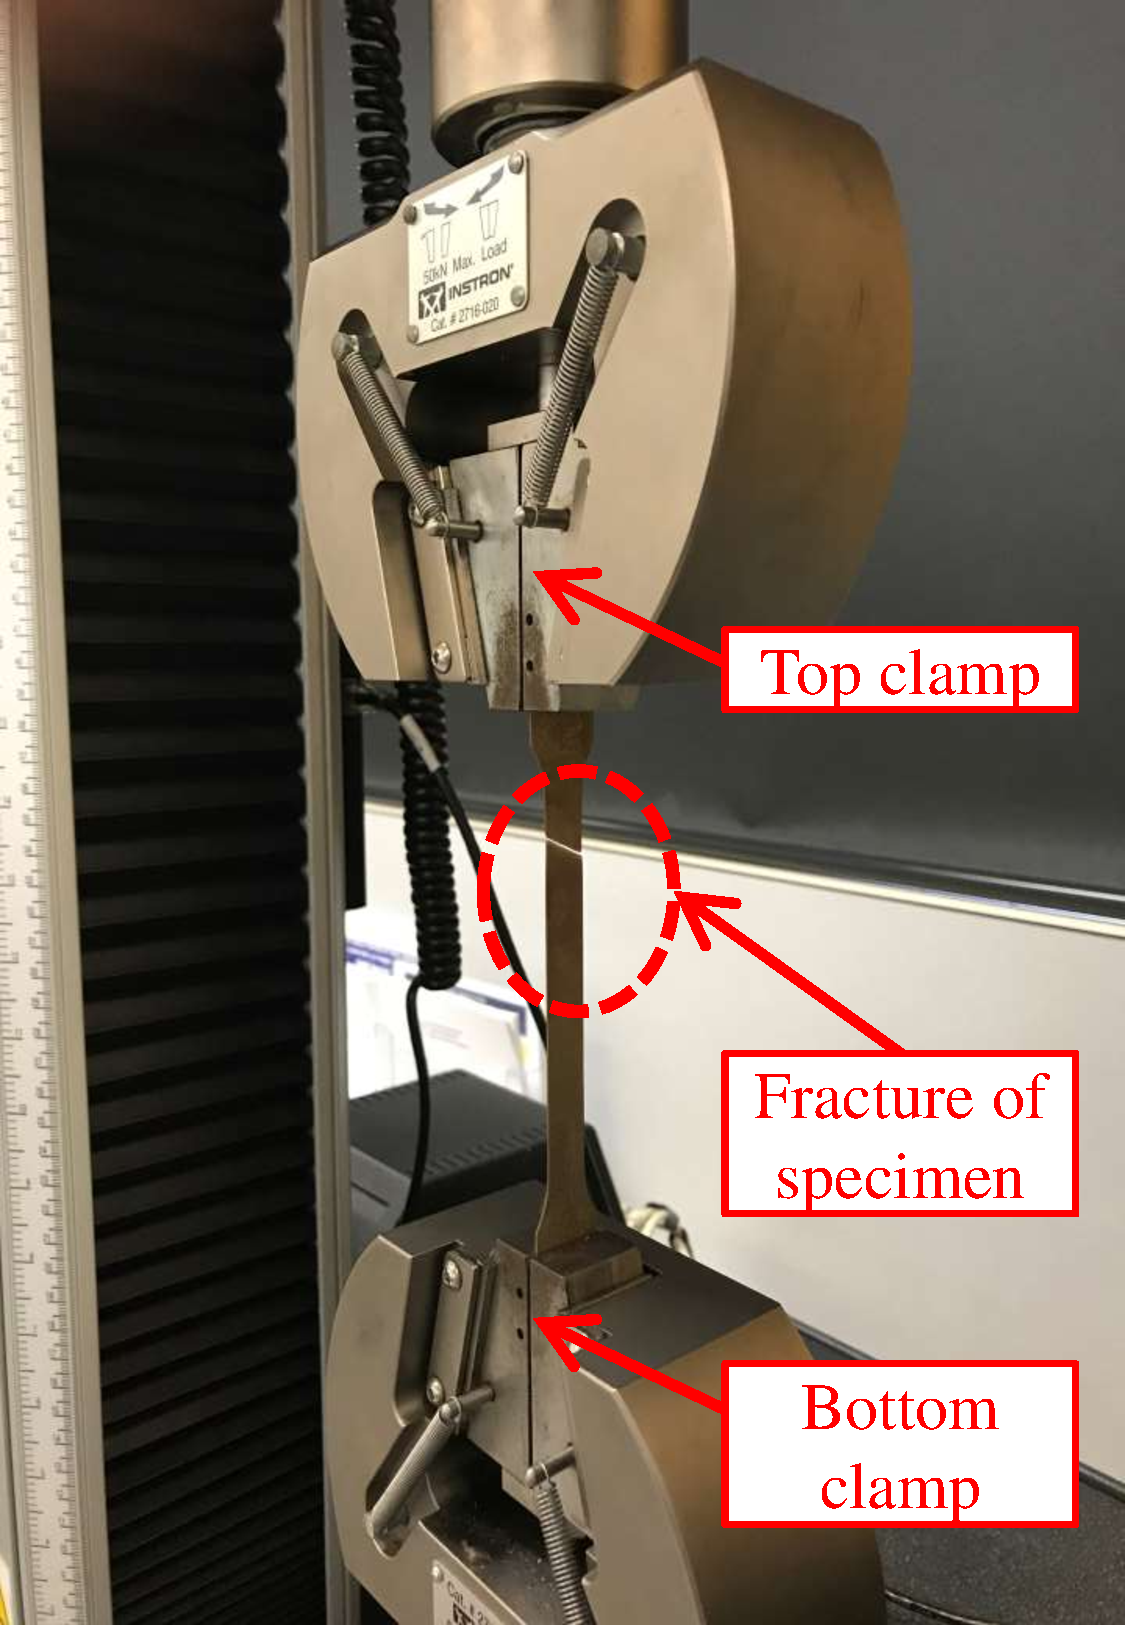
\includegraphics[width=4cm,height=6cm]{Coupon-test-setup.pdf}\\
		\caption{Tensile coupon details}
		\label{fig:tensile-coupon-test-setup}
\end{figure}
% Table generated by Excel2LaTeX from sheet '0.75'
\begin{table}[htbp]
	\centering
	\caption{Tensile coupon test results for 0.75 mm thick studs}
	  \begin{tabular}{cccc}
	  \toprule
	  \multicolumn{1}{p{2.145em}}{\centering Test\newline{}No} & 
	  \multicolumn{1}{p{4.07em}}{\centering Sample\newline{}Location} & 
	  \multicolumn{1}{p{7.07em}}{\centering Youngs\newline{}Modulus (Gpa)} & 
	  \multicolumn{1}{p{7.145em}}{\centering Yield\newline{}Strength (Mpa)} \\
	  \midrule
	  1    & Web  &  202.55 & 634.39 \\
	  2    & Web  &  232.30 & 658.45 \\
	  3    & Web  &  220.46 & 633.09 \\
	  4    & Web  &  214.28 & 642.87 \\
	  5    & Web  &  218.17 & 643.57 \\
	  6    & Web  &  212.95 & 642.92 \\
	  7    & Flange &  212.43 & 648.66 \\
	  8    & Flange &  216.45 & 658.30 \\
	  9    & Flange &  217.55 & 660.50 \\
	  \midrule
	  \multicolumn{2}{c}{Average} & 216.35 & 646.97 \\
	  \bottomrule
	  \end{tabular}%
	\label{tab:075-coupon-results}%
  \end{table}%
  % Table generated by Excel2LaTeX from sheet '0.95'

  \begin{table}[htbp]
	\centering
	\caption{Tensile coupon test results for 0.95 mm thick studs}
	  \begin{tabular}{ccccc}
	  \toprule
	  \multicolumn{1}{p{2.145em}}{\centering Test\newline{}No} & 
	  \multicolumn{1}{p{4.07em}}{\centering Sample\newline{}Location} & 
	  \multicolumn{1}{p{7.07em}}{\centering Youngs\newline{}Modulus (Gpa)} & 
	  \multicolumn{1}{p{7.145em}}{\centering Yield\newline{}Strength (Mpa)} \\
	  \midrule
	  10   & Web  &  216.50 & 612.88 \\
	  11   & Web  &  219.12 & 623.75 \\
	  12   & Web  &  202.83 & 622.87 \\
	  13   & Flange &  217.91 & 620.68 \\
	  14   & Flange &  218.56 & 620.56 \\
	  15   & Flange &  218.35 & 604.45 \\
	  \midrule
	  \multicolumn{2}{c}{Average} & 215.55 & 617.53 \\
	  \bottomrule
	  \end{tabular}%
	\label{tab:095-coupon-results}%
  \end{table}%

Tensile coupon test set up is shown in \Cref{fig:tensile-coupon-test-setup}. Details of the tensile coupon testes are presented in \Cref{tab:075-coupon-results,tab:095-coupon-results}. Total of 15 tensile coupon tests were conducted to determine the Young's Modulus and yield strength of the steel used in the ambient capacity tests. The average Young's Modulus and yield strength of 0.75 mm thick studs were 216.35 GPa and 646.97 MPa respectively. Likewise, for 0.95 mm thick steel, the average Young's Modulus and yield strength were 215.55 GPa and 617.53 MPa respectively. The yield strength of 0.75 mm thick steel was higher in comparison with 0.95 mm steel. Tensile coupons were extracted only from the stud web and flanges as these elements are most susceptible to internal stresses during the cold forming process. Tests were not conducted on the noggings and tracks as they are least susceptible to internal stresses and are not considered for the purpose of design and numerical analysis. The stress-strain curve corresponding to the specimens with the maximum Young's modulus and yield strength recorded in the web and flanges of 0.75 mm and 0.95 mm steel are shown in \Cref{fig:075-stress-strain,fig:095-stress-strain} below.
\begin{figure}
	\centering
		\begin{tabular}{cc}
			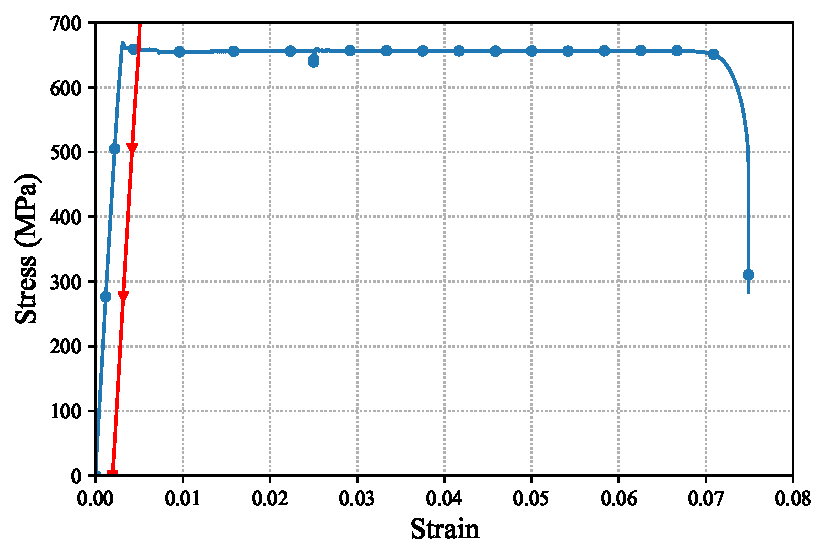
\includegraphics[width=6.5cm,height=5.5cm]{Test2-Specimen_RawData_5.pdf} & 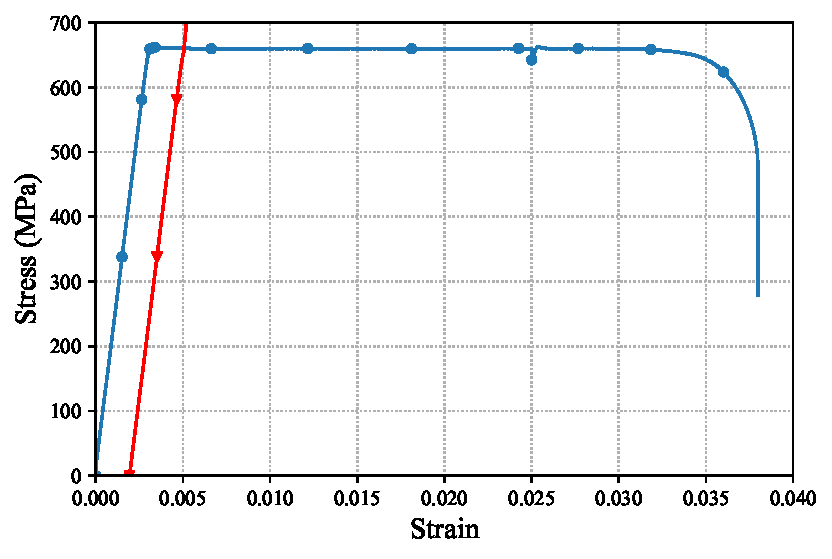
\includegraphics[width=6.5cm,height=5.5cm]{Test9-Specimen_RawData_4.pdf} \\ 
			(a) & (b)  \\ 
		\end{tabular} 
		\caption{Stress-strain curve from tensile coupon tests on 0.75 mm steel (a) Stud Web (b) Stud Flange}
		\label{fig:075-stress-strain}
\end{figure}
\begin{figure}
	\centering
		\begin{tabular}{cc}
			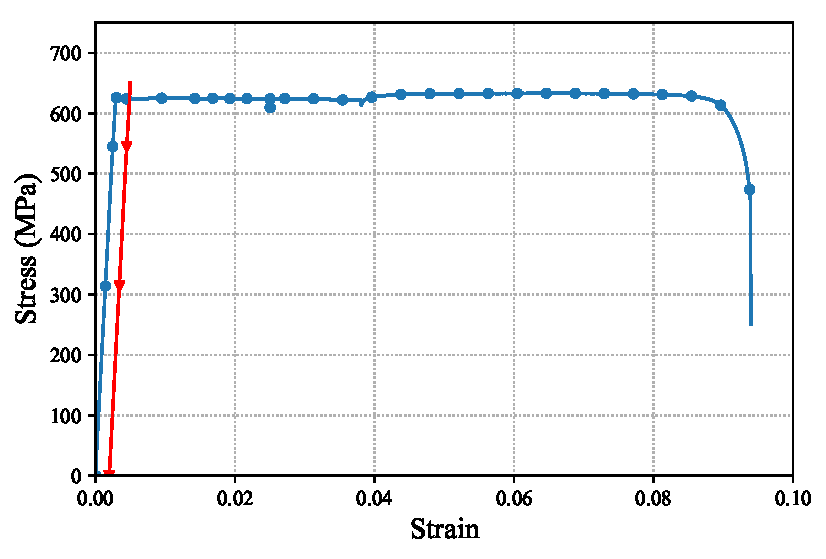
\includegraphics[width=6.5cm,height=5.5cm]{Test11-Specimen_RawData_6.pdf} & 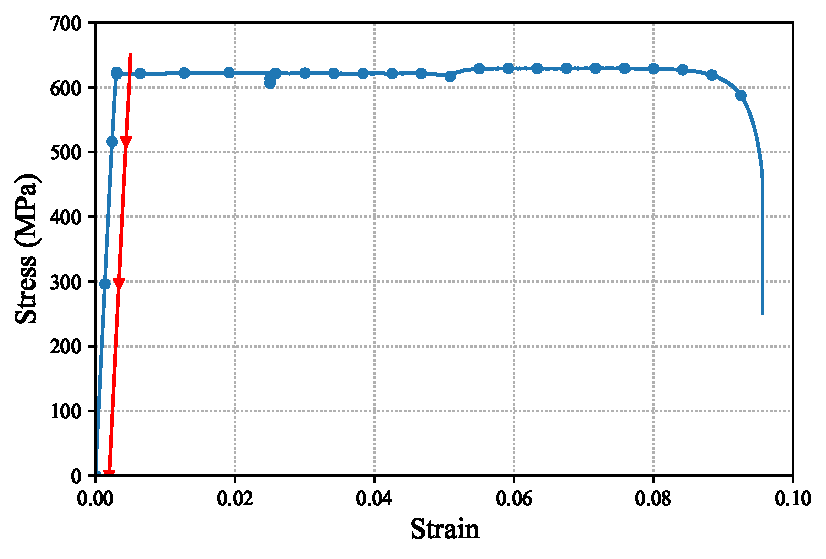
\includegraphics[width=6.5cm,height=5.5cm]{Test13-Specimen_RawData_8.pdf} \\ 
			(a) & (b)  \\ 
		\end{tabular} 
		\caption{Stress-strain curve from tensile coupon tests on 0.95 mm steel (a) Stud Web (b) Stud Flange}
		\label{fig:095-stress-strain}
\end{figure}

\section{Summary of Ambient Capacity Tests Investigations and Comparisons}

The following findings can be drawn from ambient capacity tests on single, double and staggered stud LSF walls and tensile coupon tests.
\begin{itemize}
	\item Axial compression capacity is greatly dependant on the thickness and depth of the studs.
	\item The effect of plasterboards on the stud flanges providing in-plane restraints significantly influences the axial compression capacity in single stud LSF walls. The absence of effective plasterboard restraints on the inner stud flanges in double stud walls greatly affects the axial compression capacity of double stud LSF walls.
	\item In the case of staggered stud LSF walls, despite the absence of plasterboard restraint on one flange, the omega noggings connecting the stud webs provide significant in-plane restraints to the studs resulting in a similar axial compression capacity in comparison with double stud LSF walls.
	\item The axial compression capacity of plasterboard line double stud walls are significantly higher for walls with 70 mm studs in comparison with 90 mm studs with the same thickness. This is attributed by the increased slenderness in 90 mm studs. 
	\item All the tensile coupon tests show that the minimum guaranteed yield strength of 550 MPa is achieved in all the test specimens. 0.75 mm steel resulted in higher yield strength in comparison with 0.95 mm steel despite the same grade of steel. However, the Young's Modulus remains almost similar irrespective of the thickness. This is because of the higher cold work in steel with lower thicknesses. The Young's Modulus and yield strength results from the coupon tests will later be used for numerical analysis. 
\end{itemize}
  
  
  
